\documentclass[10pt,a4paper]{article}
\usepackage[utf8]{inputenc}
\usepackage[english,russian]{babel}
\usepackage{cmap}
\usepackage[OT1]{fontenc}
\usepackage{amsmath}
\usepackage{amsfonts}
\usepackage{amssymb}
\usepackage{graphicx}
\usepackage{float}
\usepackage{wrapfig}
\usepackage{caption}
\DeclareCaptionLabelSeparator{dot}{. }
\captionsetup{justification=centering,labelsep=dot}
\graphicspath{{pictures/}}
\DeclareGraphicsExtensions{.pdf,.png,.jpg,.eps}
\begin{document}

\part{Основы}

\part{Локализация}

\textbf{7 Локализация мобильного роботы: марковские и гауссовы алгоритмы}\\

В этой главе читатель познакомится с рядом конкретных алгоритмов локализации мобильного робота. Локализация мобильного робота – это задача определения положения робота относительно данной карты окружения. Этот процесс часто называют \textit{«оценкой местоположения» (position estimation)}. Локализация мобильного робота – это частный случай задачи общей локализации, самой базовой задачей восприятия среды, поскольку практически все задачи робототехники требуют знания местоположения объектов, с которыми производятся манипуляции. Методы, описываемые в этой и последующей главах, одинаково применимы и для задач локализации объекта. 

На Рис. 7.1 показана графическая модель задачи локализации мобильного робота. Роботу дана карта окружающей среды, а его целью является определение своего положения на карте с помощью восприятия окружающей среды и оценки перемещений.

Локализацию мобильного робота можно рассматривать как проблему преобразования координат. Карты выполнены в глобальной системе координат, независимой относительно положения робота, поэтому локализацию можно свести к установлению соотношения между системой координат карты и собственной локальной системой координат робота. Знание способа преобразования координат позволяет выразить местоположение интересующих объектов в координатной системе робота, что является важным предварительным требованием для навигации. Как читатель может легко проверить, знания положения $x_t = (x\,y\,\theta)^T$ робота на карте достаточно для определения преобразования координат, при условии, что положение и карта выражены в одной и той же системе координат. 

К сожалению (в этом и состоит проблема локализации мобильного робота), положение обычно нельзя воспринять напрямую. Другими словами, большинство роботов не обладает датчиками, позволяющими без помех измерить положение. Положение приходится извлекать из данных измерений, и ключевой трудностью определения является недостаточность единственного измерения. Поэтому, чтобы определить положение, необходимо интегрировать данные измерений по времени. Чтобы понять необходимость этого, просто представим, что робот находится в здании со множеством одинаковых коридоров. В этом случае единственного измерения датчика (например, сканирования расстояния), очевидно, будет недостаточно для идентификации конкретного коридора.

\begin{figure}[H]
	\center{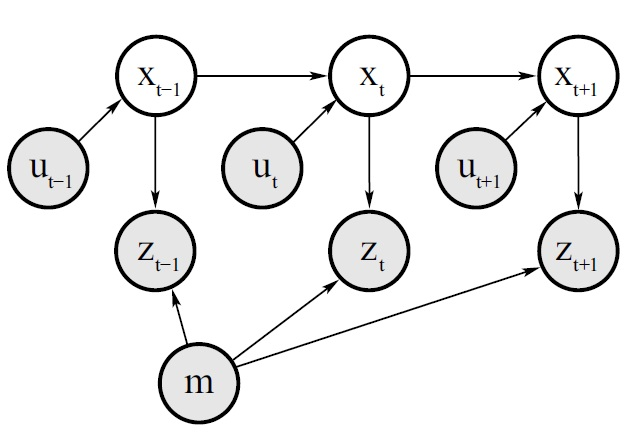
\includegraphics[width=0.85\linewidth]{71orig}}
	\caption{ (  Рис. 7.1 Графическая модель локализации мобильного робота. Значения узлов с заливкой серым цветом известны. Карта обозначена как $m$, значения измерений - $z$, а управление - $u$. Целью локализации является определение переменных положения робота $x$.
		)}
	\label{fig:71orig}
\end{figure}

Методы локализации были разработаны для широкого набора представлений карт. Мы уже обсуждали два типа карт: \textit{на основе признаков} и \textit{на основе местоположения}. Примером последних являются карты сеток занятости, которые обсуждаются в более поздней главе книги. Некоторые другие типы карт показаны на Рис. 7.2. На этой схеме показана созданная вручную метрическая двухмерная карта, топологическая карта в виде графа, карта сеток занятости и панорама из снимков потолка (которую тоже можно использовать в качестве карты). В более поздних главах будут детально описываться конкретные типы карт и обсуждаться алгоритмы получения карт из данных. Локализация подразумевает наличие точной карты. 

В этой и следующей главах будут представлены некоторые базовые вероятностные алгоритмы мобильной локализации. Все эти алгоритмы являются вариантами базового фильтра Байеса, описанного в главе 2. Мы уже обсуждали преимущества и недостатки каждого представления и соответствующих алгоритмов. В главе также излагаются некоторые обобщения, касающиеся различных проблем локализации, определённые следующей классификацией. 

\begin{figure}[H]
	\center{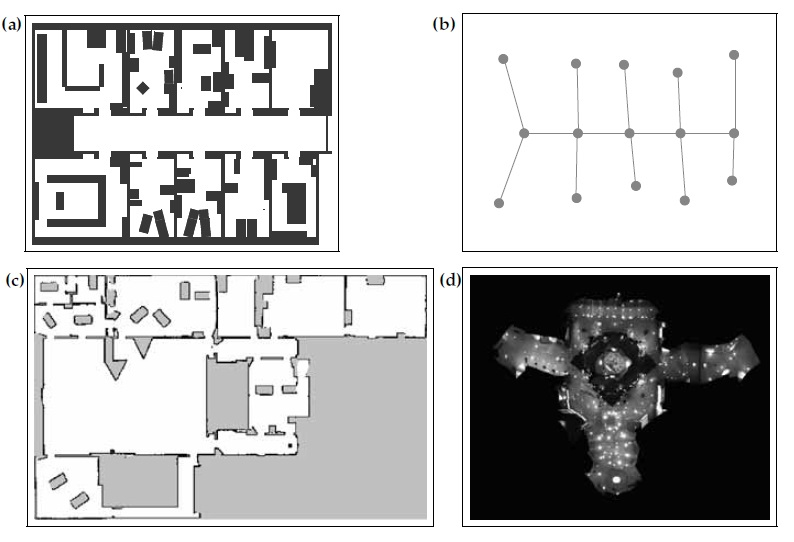
\includegraphics[width=0.87\linewidth]{72orig}}
	\caption{ (  Рис. 7.2 Примеры карт, используемых для локализации робота: двухмерная метрическая схема (a), сконструированная вручную, топологическая карта в виде графа (b), карта сетки занятости (c), и панорама изображений потолка (d). Изображения принадлежат Френку Делаэрту, из института технологий штата Джорджия (Frank Dellaert, Georgia Institute of Technology).
		)}
	\label{fig:72orig}
\end{figure}

\textbf{7.1 Классификация задач локализации}\\

Не все проблемы локализации одинаково трудны и для понимания необходимо кратко обсудить их классификацию. В этой классификации проблемы разделены по ряду важных критериев, касающихся природы окружающей среды и начальной информации, которой может обладать робот.\\

\textbf{Локальная локализация против глобальной} 
Проблемы локализации характеризуются типом осведомлённости, доступной изначально и при работе. Определим три типа проблем локализации с возрастающей сложностью.\\ 
ОТСЛЕЖИВАНИЕ ПОЗИЦИИ 

\textit{Отслеживание положения} подразумевает, что \textit{начальное положение} робота известно. Локализация робота может быть достигнута, если суметь приспособиться к шумам при движении робота. Эффект таких шумов обычно достаточно мал, поэтому методы отслеживания позиции часто полагаются на допущение о малой ошибке положения. Неопределённость положения часто аппроксимируется одномодальным распределением (например, гауссовым). Проблема отслеживания позиции – локальная, поскольку неопределённость носит локальный характер и ограничена областью вблизи истинного положения робота.\\
ГЛОБАЛЬНАЯ ЛОКАЛИЗАЦИЯ

В \textit{глобальной локализации}, первоначальное положение робота неизвестно. Изначально, робот  помещён в некотором месте окружающей среды, но нет никаких данных ни о его местоположении, ни о самом окружении нет. Методы глобальной локализации не могут ограничиваться одной лишь ошибкой положения. Как позже будет показано в этой главе, одномодальные вероятностные распределения также обычно неприменимы. Глобальная локализация более трудна, чем отслеживание позиции, и включает в себя задачу отслеживания как составную часть.\\ 
ПРОБЛЕМА ПОХИЩЕННОГО РОБОТА

\textit{Проблема похищенного робота} является вариантом проблемы глобальной локализации, но ещё более трудна. Представим, что работающий робот был похищен и телепортирован в какое-то другое место. Дополнительная сложность по сравнению с проблемой глобальной локализации, состоит в том, что робот может ошибочно предполагать, что знает своё текущее положение. В глобальной локализации роботу всегда известно, что начальное местоположение неизвестно. Можно оспорить эту точку зрения и сказать, что на практике роботов похищают довольно редко. Практическая важность этой проблемы состоит в том, что даже самые современные алгоритмы локализации не защищены от сбоев, а возможность восстанавливаться после возникновения ошибки по-настоящему важна для автономных роботов. Тестирование алгоритма локализации «имитацией похищения» позволяет проверить его способность восстанавливаться после сбоя глобальной локализации. \\

\textbf{Статическое и динамическое окружение} Вторым фактором, оказывающим существенное влияние на локализацию, является окружающая среда. Окружение может быть статическим или динамическим.\\
СТАТИЧЕСКОЕ ОКРУЖЕНИЕ 

\textit{Статическая окружающая среда} – это такая среда, где единственным изменяющимся значением (состоянием) является положение робота. Другими словами, в статической среде движется только робот, а все другие объекты среды всегда остаются на своих местах. Статические среды имеют некоторые математические свойства, облегчающие эффективную вероятностную оценку.\\ 
ДИНАМИЧЕСКОЕ ОКРУЖЕНИЕ

\textit{Динамическая окружающая среда} содержит объекты, помимо самого робота, местоположение или конфигурация которых изменяется со временем. Особенный интерес представляют изменения, которые сохраняются со временем и влияют более чем на одно измерение датчика. 
Изменения, которые невозможно измерить, конечно, не имеют отношения к локализации, а те, что затрагивают единственное измерение, лучше всего считать шумами. (см подраздел 2.4.4). Примерами более постоянных воздействий являются: наличие людей, засветки (для роботов, оборудованных камерами), перемещений мебели или дверей. Очевидно, что большинство реальных окружающих сред динамические, с изменениями состояния, происходящими в различных диапазонах скоростей. 

Очевидно, локализация в динамических средах более трудна, чем в статических. Есть два принципиальных подхода к обработке динамики. Во-первых, динамические элементы можно включить в вектор состояний. В результате, марковское свойство снова будет соблюдаться, но такой подход влечёт за собой увеличение вычислительной и модельной сложности. Во–вторых, в некоторых ситуациях данные датчиков можно подвергнуть фильтрации, чтобы уничтожить негативные эффекты не смоделированной динамики. Такой подход описан ниже в подразделе 8.4.\\

\textbf{Пассивный и активный подход} Третий параметр, характеризующий проблемы локализации, связан с тем, управляет ли алгоритм локализации движением робота. Можно выделить два класса:\\
ПАССИВНАЯ ЛОКАЛИЗАЦИЯ 

При \textit{пассивной локализации} модуль локализации только наблюдает за действиями робота, а управление роботом осуществляется какими-то иными методами. Движение не используется в локализации и робот может перемещаться случайным образом или же выполнять какие-то регулярные действия.\\ 
АКТИВНАЯ ЛОКАЛИЗАЦИЯ 

Алгоритмы \textit{активной локализации} управляют роботом таким образом, чтобы минимизировать ошибку локализации и/или ущерб, причинённый ошибочным перемещением робота в опасное место. 

Активный подход к локализации обычно показывает лучшие результаты локализации по сравнению с пассивным и мы уже обсуждали подобный пример прибрежной навигации во вводной части книги. Второй пример показан на Рис. 7.3. Здесь робот расположен в симметричном коридоре, и оценка после навигации по коридору сходится к двум (симметричным) положениям. Локальная симметрия среды делает невозможной локализацию робота в коридоре, и определение положения возможно только после захода в комнату и разрешения неопределённости состояния. Именно в таких ситуациях активная локализация даёт лучшие результаты, поскольку вместо того, чтобы просто ждать, пока робот случайно войдёт в комнату, возможно вовремя спрогнозировать безвыходную ситуацию, что позволит её предотвратить. 

Главным ограничением активных методов является необходимость наличия возможности управлять роботом. На практике это требование делает использование одной лишь активной локализации недостаточным, поскольку роботу необходимо определять своё местоположение даже в процессе выполнении какой-либо задачи. Некоторые методы активной локализации создаются на основе пассивных методов. Другие комбинируют выполнение основной задачи с задачей локализации при управлении роботом. 

\begin{figure}[H]
	\center{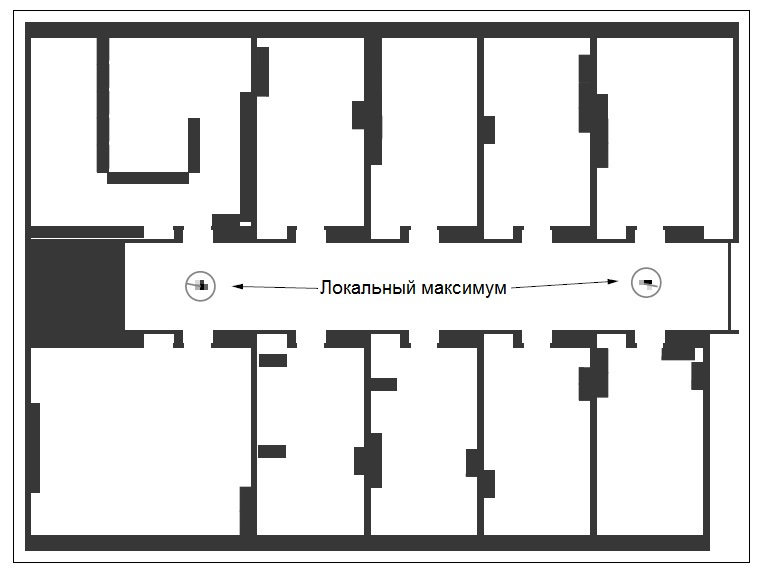
\includegraphics[width=0.87\linewidth]{73orig}}
	\caption{ (  Рис. 7.3 Модельная ситуация, иллюстрирующая типичную оценку состояния при выполнении глобальной локализации в локально симметричной среде. Роботу необходимо зайти в комнату для определения своего местоположения. 	)}
	\label{fig:73orig}
\end{figure}

В этой главе описаны исключительно алгоритмы пассивных методов локализации. Активная локализация будет обсуждаться в главе 17.\\

\textbf{Один или несколько роботов} Четвёртым критерием проблемы локализации является количество задействованных роботов.\\ 
ЛОКАЛИЗАЦИЯ ОДИНОЧНЫМ РОБОТОМ

\textit{Локализация одиночным роботом} наиболее часто встречается в локализации и имеет дело с единственным роботом. В этом случае предполагается, что все данные собираются с помощью единственной робототехнической платформы и любая коммуникация отсутствует.\\ 
ЛОКАЛИЗАЦИЯ НЕСКОЛЬКИХ РОБОТОВ

Задача \textit{локализации нескольких роботов} возникает в группах роботов. На первый взгляд, каждый робот может локализовать себя самостоятельно, поэтому проблема локализации несколькими роботами может быть решена через локализацию одним роботом. Но, если роботы в состоянии обнаружить друг друга, имеется лучшая возможность. 
Дело в том, что при известных относительных местоположениях нескольких роботов оценка одного робота может быть использована, чтобы уточнить оценку местоположения другого робота. Для случая локализации нескольких роботов возникают интересные и нетривиальные соображения относительно отображения оценок и природы связи между ними. 

Эти четыре критерия отражают наиболее важные характеристики проблемы локализации мобильных роботов.

\begin{table}[H]
\begin{center}
\begin{tabular}{|l|}
\hline
{}\\
1: \hspace{3mm} Algorithm Markov\_localization $(bel(x_{t-1}),u_t,z_t,m):$ \\
2:\hspace{7mm}$\textit{for all}\, x_t\,\textit{do}$\\
3:\hspace{12mm}$\overline{bel}(x_t)=\int p(x_t|u_t,x_{t-1},m)bel(x_{t-1})dx_{t-1}$\\
4:\hspace{12mm}$bel(x_t)=\eta\,p(z_t|x_t,m)\overline{bel}(x_t)$\\
5:\hspace{7mm}$\textit{endfor}$\\
9:\hspace{7mm}$\textit{return}\,bel(x_t)$\\
{}\\
\hline
\end{tabular}
\caption{(Таблица 7.1 Марковская локализация.)}
	\end{center}
\end{table}

Существуют и другие характеристики, влияющие на сложность проблемы, такие, как информация, полученная из измерений и её утрата при передвижении робота.
Кроме того, симметричные среды более трудны для выполнения локализации, чем асимметричные из-за более высокой степени возникающей неоднозначности. 

\textbf{7.2 Марковская локализация}\\

Вероятностные алгоритмы локализации являются вариантами фильтра Байеса. Непосредственное приложение байесовских фильтров к проблеме локализации называется \textit{марковской локализацией}. В Таблице 7.1 описан основной алгоритм. Этот алгоритм выведен из \textbf{Bayes\_filter} (Таблица 2.1 на странице 27???????). Заметим, что для алгоритма \textbf{Markov\_localization} также требуется карта $m$ в качестве входных данных, которая используется в модели измерений $p(z_t | x_t, m)$ (строка 4). Она часто, хотя и не всегда, также включается в модель движения $p(x_t | u_t, x_{t-1}, m)$ (строка 3). Также, как и байесовский фильтр, марковская локализация преобразует вероятностную оценку в момент времени $t - 1$ в оценку в момент времени $t$. С помощью марковской локализации возможно решать задачи глобальной локализации, отслеживания позиции и украденного робота в статических средах. 

Начальная оценка $bel(x_0)$ отражает исходную степень осведомлённости относительно положения робота.
Она устанавливается различными способом, зависящим от типа задачи локализации.\\

• \textbf{Отслеживание позиции}. Если известно начальное положение, $bel(x_0)$ инициализируется распределением, сосредоточенным в одной точке. Пусть $\bar{x}_0$ означает (известное) начальное положение. Тогда\\

(7.1)
\begin{equation*}
bel(x_0)=\left\{
\begin{array}{ll}
1 & \mbox{ если } x_0=\bar{x}_0\\
0 & \mbox{в других случаях}\\
\end{array}
\right.
\end{equation*}

Точечные распределения дискретны и плотностью не обладают.  

\begin{figure}[H]
	\center{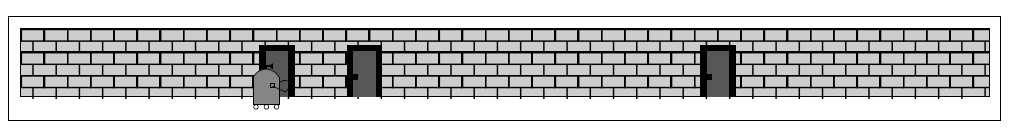
\includegraphics[width=1\linewidth]{74orig}}
	\caption{ (  Рис. 7.4 Модельная среда для иллюстрации локализации мобильного робота: одномерный коридор с тремя неразличимыми между собой дверьми. Изначально робот не знает своего местоположения, только направление движения, и его целью является выполнение локализации.)}
	\label{fig:74orig}
\end{figure}

На практике начальное положение часто известно лишь приблизительно. В этом случае оценка $bel(x_0)$  инициализируется узким нормальным распределением с центром около $\bar{x}_0$. Нормальные распределения определены выражением (2.4) на странице 15????.\\

(7.2)
$$bel(x_0)=\underbrace{\det(2\pi\varSigma)^{-\frac{1}{2}}\exp\{-\frac{1}{2}(x_0-\bar{x}_0)^T\varSigma^{-1}(x_0-\bar{x}_0)\}}_{\sim \mathcal{N}(x_0;\bar{x}_0,\varSigma)}$$

$\varSigma$–это ковариация неопределённости начального положения.\\

• \textbf{Глобальная локализация}. Если начальное положение неизвестно, $bel(x_0)$ инициализируется равномерным распределением в пространстве всех допустимых положений карты:\\

(7.3)
$$bel(x_0)=\frac{1}{|X|}$$

где $|X|$ означает объем (мера Лебега) пространства всех положений на карте.\\

• \textbf{Прочие}. Частичное понимание роботом своей позиции обычно может быть легко преобразовано в применимое первичное распределение. Например, если известно, что робот стартует около двери, можно инициализировать $bel(x_0)$  нулевой плотностью, кроме мест около двери, где она может быть однородной. Если известно, что робот находится в конкретном коридоре, можно инициализировать $bel(x_0)$ однородным распределением в коридоре и нулём во всех остальных точках.\\

\textbf{7.3 Иллюстрация марковской локализации}\\

Мы уже обсуждали марковскую локализацию во вводной части книги в качестве иллюстративного примера вероятностной робототехники. Сейчас мы можем вернуться к примеру, используя математический подход. На Рис. 7.4 показан одномерный коридор с тремя идентичными дверями. Первичная гипотеза $bel(x_0)$ равномерна для всех положений, что показано на Рис. 7.5a равномерной плотностью. Когда робот запрашивает датчики и обнаруживает, что находится около одной из дверей, происходит умножение оценки $bel(x_0)$ на $p(z_t | x_t, m)$, как показано в строке 4 алгоритма. На верхней плотности на Рис. 7.5b показана вероятность $p(z_t | x_t, m)$ для примера с коридором. Нижняя плотность является результатом умножения этой плотности на априорную равномерную гипотезу. Здесь снова получается многомодовая результирующая гипотеза, отражающая остаточную неопределённость в этой точке.

\begin{figure}[H]
	\center{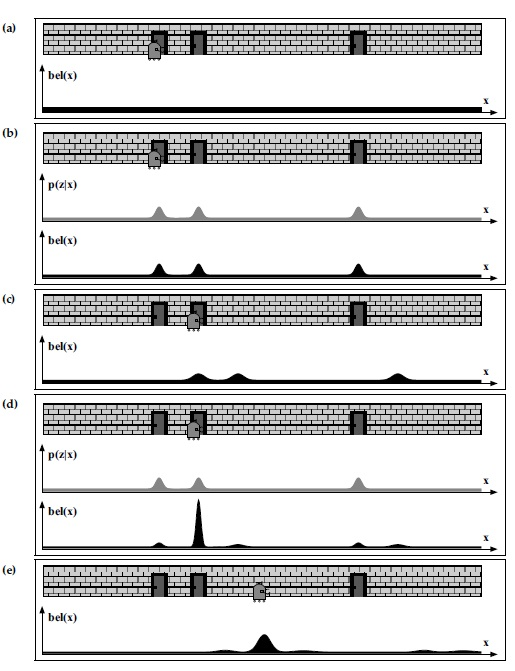
\includegraphics[width=0.95\linewidth]{75orig}}
	\caption{ (  Рис. 7.5 Иллюстрация марковского алгоритма локализации. На каждой схеме показана позиция робота в коридоре и текущая гипотеза $bel(x)$. На схемах (b) и (d) также показана модель наблюдений $p(z_t | x_t)$, описывающая вероятность наблюдения двери в разных местоположениях коридора.)}
	\label{fig:75orig}
\end{figure} 

По мере того, как робот перемещается вправо, как показано на Рис. 7.5c, в строке 3 марковского алгоритма локализации происходит свёртка оценки с моделью движения $p(x_t | u_t, x_{t-1})$. Модель движения $p(x_t | u_t, x_{t-1})$ не сосредоточена на одном положении, но распределена на всем континууме положений с центром вокруг ожидаемого результата идеального движения. Результат приведён на Рис. 7.5c, где показано смещение оценки, которая также расширена в результате выполнения свёртки. 

Последнее измерение показано на Рис. 7.5d. Здесь в алгоритме марковской локализации выполняется перемножение текущей гипотезы с вероятностью восприятия $p(z_t | x_t)$. На этой точке большая часть вероятности сфокусирована около истинного расположения и робот достаточно уверен, что сумел выполнить локализацию. 
На Рис. 7.5e показана гипотеза робота после передвижения вниз по коридору. 

Уже было замечено, что марковская локализация не зависит от основного отображения пространства состояний. Фактически, её возможно реализовать, используя любое из отображений, обсуждаемых в Главе 2. Давайте выведем практические алгоритмы, способные локализовать робота в реальном времени, используя три различных отображения. Начнём с фильтров Калмана, в которых  гипотеза отображается в виде первого и второго моментов. Затем продолжим рассмотрение с дискретными, сеточными представлениями и, наконец, представим алгоритмы на основе многочастичных фильтров.\\

\textbf{7.4 Локализация на основе EKF}\\

Алгоритм  \textit{локализации на основе обобщённых фильтров Калмана} или \textit{локализация на основе EKF} – это особый случай марковской локализации. Локализация на основе EKF отображает гипотезы $bel(x_t)$ в виде первого и второго моментов, математического ожидания $\mu_t$ и ковариации $\varSigma_t$. Базовый алгоритм EKF приведён в Таблице 3.3 в Главе 3.3 (страница 59???????). Локализация на основе EKF будет нашей первой практической реализацией EKF в контексте настоящей задачи робототехники. 

Наш алгоритм локализации EKF подразумевает, что карта отображается в виде набора признаков. В любой момент времени $t$, робот может принимать вектор расстояний и направлений на близлежащие признаки: $z_t = \{z_t^1, z_t^2, . . .\}$. Начнём с алгоритма локализации, в котором все признаки уникально различимы.
Существование уникально различимых признаков необязательно является плохим допущением. Например, Эйфелева башня в Париже – это ориентир, который сложно перепутать с чем-то ещё и она хорошо видима со многих точек Парижа.\\
ПЕРЕМЕННАЯ СООТВЕТСТВИЯ

Обозначим признаки набором \textit{переменных соответствия} $c^i_t$, по одной для каждого вектора признаков $z^i_t$. Переменные соответствия также уже обсуждались в Главе 6.6. Для начала допустим, что соответствия известны. Затем разовьём изложение до более общего случая, позволяющего использовать неразличимые признаки. В более общем случае для оценки значения латентной переменной соответствия будет использоваться алгоритм максимального правдоподобия, а результат этой оценки - использован в качестве эталонного.\\

\textbf{7.4.1 Иллюстрация} \\

На Рис. 7.6 показан алгоритм локализации на основе EKF, для примера локализации мобильного робота в одномерном коридоре (см. Рис. 7.4). В целях удобства и для обеспечения одномодальной формы гипотезы распределения в EKF, сделаем два допущения. Во-первых, допустим, что соответствия известны. Присвоим уникальные метки дверям (1, 2 и 3), и определим модель измерений $p(z_t | x_t, m, c_t)$, где $m$  это карта, а $c_t\in\{1, 2, 3\}$ обозначает двери, наблюдаемые в момент времени $t$. Во-вторых, допустим, что начальное положение относительно хорошо известно. Типичная начальная оценка в виде нормального распределения, показанная на Рис. 7.6a, имеет центр в зоне около Двери 1 и гауссовскую  неопределённость. По мере движения робота вправ, выполняется свёртка оценки вместе с моделью движения. Результирующей оценкой является смещённая гауссовская функция с увеличенной шириной, показанная на Рис.7.6b.

\begin{figure}[H]
	\center{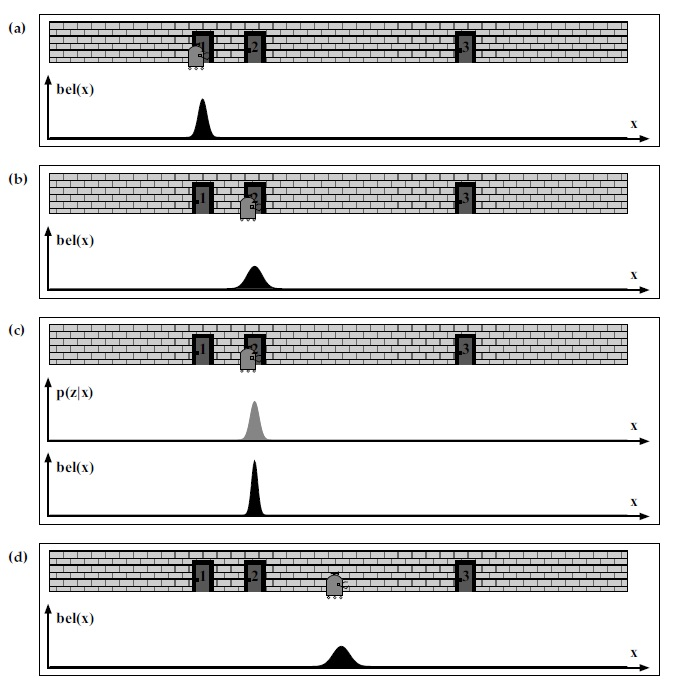
\includegraphics[width=1\linewidth]{76orig}}
	\caption{ (  Рис. 7.6 Применение алгоритма фильтра Калмана для локализации мобильного робота. Все плотности представлены одномодальными гауссовыми функциями.)}
	\label{fig:76orig}
\end{figure}

Теперь допустим, что робот обнаружил, что находится около двери $c_t = 2$. Верхняя плотность на Рис 7.6c показывает $p(z_t | x_t, m, c_t)$ для этого наблюдения (снова в виде гауссового распределения). Свёрткой вероятности измерения в оценку робота получается апостериорная вероятность, показанная на Рис. 7.6c. Стоит заметить, что дисперсия результирующей оценки меньше, чем для обоих предыдущих наблюдений и плотности наблюдения. Это естественно, поскольку интегрирование двух независимых оценок позволяет уточнить оценку робота, по сравнению с любой из отдельных оценок. После перемещения вниз по коридору неопределённость робота в оценке местоположения снова возрастает, поскольку EKF продолжает добавлять её (Рис. 7.6d). Этим примером можно наглядно проиллюстрировать использование фильтра Калмана в ограниченных условиях задачи.\\

\textbf{7.4.2 Алгоритм локализации EKF}\\ 

До настоящего момента дискуссия носила довольно абстрактный характер. По умолчанию считалось, что подходящие модели движения и измерения доступны, а количество ключевых переменных для обновления EKF не было определено. Давайте обсудим конкретную реализацию EKF для карт на основе признаков, состоящих из точечных ориентиров, как уже обсуждалось в подразделе 6.2.
Для таких точечных ориентиров используем обычную модель измерений, обсуждаемую в подразделе 6.6. Также используем модель движения на основе скорости, определённую в подразделе 5.3. Перед тем, как продолжать чтение, читателю рекомендуется ненадолго вернуться к указанным разделам, чтобы восстановить основные уравнения измерения и движения.

В Таблице 7.2 описан алгоритм локализации на основе EKF с известными соотношениями \textbf{EKF\_localization\_known\_correspondences}. Этот алгоритм выводится из EKF в Таблице 3.3 Главы 3. На вход принимается гауссова оценка положения робота в момент времени $t - 1$, с математическим ожиданием $\mu_{t-1}$ и ковариацией $\varSigma_{t-1}$. Далее, требуется управляющее воздействие $u_t$, карта $m$, и набор переменных $z_t = \{z_t^1, z_t^2, . . .\}$, измеренных в момент времени $t$, вместе с переменными соответствия $c_t = \{c^1_t , c^2_t , . . .\}$. На выход возвращается новое значение $\mu_t$, $\varSigma_t$, а также правдоподобие наблюдения признака $p_{z_t}$. Алгоритм не обрабатывает случай прямолинейного движения, для которого $\omega_t = 0$. Обработку этого случая оставим для рассмотрения читателю в качестве упражнения.

Отдельные вычисления в этом алгоритме описаны ниже.
В строках 3 и 4 вычисляются якобианы, необходимые для линеаризованной модели движения.
В строке 5 из данных управления определяется матрица ковариации шумов движения. В строках 6 и 7 реализуется уже знакомое обновление движения. Прогнозируемое положение после окончания движения $\bar{\mu}_t$ вычисляется в строке 6, а в строке 7 – соответствующий эллипс неопределённости. Обновление измерения (шаг коррекции) реализован в строках с 8 по 21. Основой такта обновления является перебор в цикле $i$ всех признаков, наблюдаемых в момент времени $t$. В строке 10 назначается $j$-е соответствие $i$-му признаку в векторе измерений, а затем вычисляется прогнозируемое измерение $\hat{z}_t^i$ и якобиан $H_t^i$ модели измерения.

\begin{table}[H]
\begin{center}
\begin{tabular}{|l|}
\hline
{}\\
1: Algorithm EKF\_localization\_known\_correspondences$(\mu_{t-1},\varSigma_{t-1},u_t,z_t,c_t,m):$ \\
2:\hspace{5mm}$\theta=\mu_{t-1,\theta}$\\
3:\hspace{5mm}
\begin{minipage}{0.2\textwidth}
\begin{equation*}
G_t=
\left(\begin{array}{ccc}
1&0&-\frac{\upsilon_t}{\omega_t}\cos\theta+\frac{\upsilon_t}{\omega_t}\cos(\theta+\omega_t\varDelta t)\\
0&1&-\frac{\upsilon_t}{\omega_t}\sin\theta+\frac{\upsilon_t}{\omega_t}\sin(\theta+\omega_t\varDelta t)\\
0&0&1\\
\end{array}\right)
\end{equation*}
\end{minipage}\\
4:\hspace{5mm}
\begin{minipage}{0.2\textwidth}
\begin{equation*}
V_t=
\left(\begin{array}{cc}
\frac{-\sin\theta+\sin(\theta+\omega_t\varDelta t)}{\omega_t}&\frac{\upsilon_t(\sin\theta-\sin(\theta+\omega_t\varDelta t))}{\omega_t^2}+\frac{\upsilon_t\cos(\theta+\omega_t\varDelta t)\varDelta t}{\omega_t}\\
\frac{\cos\theta-\cos(\theta+\omega_t\varDelta t)}{\omega_t}&-\frac{\upsilon_t(\cos\theta-\cos(\theta+\omega_t\varDelta t))}{\omega_t^2}+\frac{\upsilon_t\sin(\theta+\omega_t\varDelta t)\varDelta t}{\omega_t}\\
0&\varDelta t\\
\end{array}\right)
\end{equation*}
\end{minipage}\\
5:\hspace{5mm}
\begin{minipage}{0.2\textwidth}
\begin{equation*}
M_t=
\left(\begin{array}{cc}
\alpha_1\upsilon_t^2+\alpha_2\omega_t^2&0\\
0&\alpha_3\upsilon_t^2+\alpha_4\omega_t^2\\
\end{array}\right)
\end{equation*}
\end{minipage}\\
6:\hspace{5mm}
\begin{minipage}{0.2\textwidth}
\begin{equation*}
\bar{\mu}_t=\mu_{t-1}+
\left(\begin{array}{c}
-\frac{\upsilon_t}{\omega_t}\sin\theta+\frac{\upsilon_t}{\omega_t}\sin(\theta+\omega_t\varDelta t)\\
\frac{\upsilon_t}{\omega_t}\cos\theta-\frac{\upsilon_t}{\omega_t}\cos(\theta+\omega_t\varDelta t)\\
\omega_t\varDelta t\\
\end{array}\right)
\end{equation*}
\end{minipage}\\
7:\hspace{5mm}$\bar{\varSigma}_t=G_t\varSigma_{t-1}G_t^T+V_tM_tV_t^T$\\
8:\hspace{5mm}
\begin{minipage}{0.2\textwidth}
\begin{equation*}
Q_t=
\left(\begin{array}{ccc}
\sigma^2_r&0&0\\
0&\sigma^2_\phi&0\\
0&0&\sigma^2_s\\
\end{array}\right)
\end{equation*}
\end{minipage}\\
9:\hspace{6mm}$\textit{for all observed features}\,z_t^i=(r_t^i\,\phi_t^i\,s_t^i)^T\textit{do}$\\
10:\hspace{12mm}$j=c_t^i$\\
11:\hspace{12mm}$q=(m_{j,x}-\bar{\mu}_{t,x})^2+(m_{j,y}-\bar{\mu}_{t,y})^2$\\
12:\hspace{12mm}
\begin{minipage}{0.2\textwidth}
\begin{equation*}
\hat{z}_t^i=
\left(\begin{array}{c}
\sqrt{q}\\
\text{atan}2(m_{j,y}-\bar{\mu}_{t,y},m_{j,x}-\bar{\mu}_{t,x})-\bar{\mu}_{t,\theta}\\
m_{j,s}\\
\end{array}\right)
\end{equation*}
\end{minipage}\\
13:\hspace{12mm}
\begin{minipage}{0.2\textwidth}
\begin{equation*}
H_t^i=
\left(\begin{array}{ccc}
-\frac{m_{j,x}-\bar{\mu}_{t,x}}{\sqrt{q}}&-\frac{m_{j,y}-\bar{\mu}_{t,y}}{\sqrt{q}}&0\\
\frac{m_{j,y}-\bar{\mu}_{t,y}}{q}&-\frac{m_{j,x}-\bar{\mu}_{t,x}}{q}&-1\\
0&0&0\\
\end{array}\right)
\end{equation*}
\end{minipage}\\
14:\hspace{12mm}$S_t^i=H_t^i\bar{\varSigma}_t[H_t^i]^T+Q_t$\\
15:\hspace{12mm}$K_t^i=\bar{\varSigma}_t[H_t^i]^T[S_t^i]^{-1}$\\
16:\hspace{12mm}$\bar{\mu}_t=\bar{\mu}_t+K_t^i(z_t^i-\hat{z}_t^i)$\\
17:\hspace{12mm}$\bar{\varSigma}_t=(I-K_t^i\,H_t^i)\bar{\varSigma}_t$\\
18:\hspace{4mm}$\textit{endfor}$\\
19:\hspace{4mm}$\mu_t=\bar{\mu}_t$\\
20:\hspace{4mm}$\varSigma_t=\bar{\varSigma}_t$\\
21:\hspace{4mm}$p_{z_t}=\prod_i \det(2\pi S_t^i)^{-\frac{1}{2}}\exp\{-\frac{1}{2}(z_t^i-\hat{z}_t^i)^T[S_t^i]^{-1}(z_t^i-\hat{z}_t^i)\}$\\
22:\hspace{4mm}$\textit{return}\,\mu_t,\varSigma_t,p_{z_t}$\\
{}\\
\hline
\end{tabular}
\caption{(Таблица 7.2 Алгоритм локализации с помощью обобщённого фильтра Калмана (EKF), сформулированного для карты на основе признаков и робота с датчиком измерения расстояния и направления. Эта версия подразумевает знание точных значений соответствия.)}
\end{center}
\end{table}

 Используя этот якобиан, вычисляется $S_t^i$, то есть неопределённость прогнозируемого измерения $\hat{z}_t^i$. Усиление Калмана $K_t^i$ вычисляется в строке 15. Обновление оценки выполняется в строках 16 и 17, единожды для каждого признака. В строках 19 и 20 устанавливается новая оценка положения, за которой следует вычисление правдоподобия измерения в строке 21. В этом алгоритме следует обращать внимание на разницу углов, поскольку результат может выйти за пределы $2\pi$.\\
 
\textbf{7.4.3 Математический вывод локализации с помощью EKF }\\

\textbf{Шаг экстраполяции (Строки 3–7)} В алгоритме локализации EKF используется модель движения, определённая уравнением (5.13). Кратко повторим определение:\\

(7.4) 
\begin{minipage}{0.2\textwidth}
	\begin{equation*}
	\left(\begin{array}{c}
	x'\\
	y'\\
	\theta'\\
	\end{array}\right)
	=
	\left(\begin{array}{c}
	x\\
	y\\
	\theta\\
	\end{array}\right)
	+
	\left(\begin{array}{c}
    -\frac{\hat{\upsilon}_t}{\hat{\omega}_t}\sin\theta+\frac{\hat{\upsilon}_t}{\hat{\omega}_t}\sin(\theta+\hat{\omega}_t\varDelta t)\\
	\frac{\hat{\upsilon}_t}{\hat{\omega}_t}\cos\theta-\frac{\hat{\upsilon}_t}{\hat{\omega}_t}\cos(\theta+\hat{\omega}_t\varDelta t)\\
    \hat{\omega}_t\varDelta t\\
	\end{array}\right)
	\end{equation*}
\end{minipage}\\ 

Здесь $x_{t-1} = (x\,y\,\theta)^T$ и $x_t = (x'\,y'\,\theta')^T$ выражают векторы состояния в момент времени $t - 1$ и $t$, соответственно. Истинное движение описано поступательной скоростью
$\hat{\upsilon}_t$, и вращательной скоростью $\hat{\omega}_t$. Как уже было указано в уравнении (5.10), эти скорости генерируются сигналами управления перемещением, $u_t = (v_t\, \omega_t)^T$, с добавленным гауссовым шумом:\\

(7.5)
\begin{minipage}{0.2\textwidth}
	\begin{equation*}
	\left(\begin{array}{c}
	\hat{\upsilon}_t\\
	\hat{\omega}_t\\
	\end{array}\right)
	=
	\left(\begin{array}{c}
	\upsilon_t\\
	\omega_t\\
	\end{array}\right)
	+
	\left(\begin{array}{c}
	\varepsilon_{\alpha_1\upsilon_t^2+\alpha_2\omega_t^2}\\
	\varepsilon_{\alpha_3\upsilon_t^2+\alpha_4\omega_t^2}\\
	\end{array}\right)
	=
	\left(\begin{array}{c}
	\upsilon_t\\
	\omega_t\\
	\end{array}\right)
	+\mathcal{N}(0,M_t)
	\end{equation*}
\end{minipage}\\

Из Главы 3 известно, что для локализации с помощью EKF поддерживается локальная апостериорная оценка состояния, выраженная в виде математического ожидания $\mu_{t-1}$ и ковариации $\varSigma_{t-1}$. Также вспомним, что базовым свойством EKF является линеаризации модели движения и измерения. Разложим модель движения на идеальную часть и случайный компонент шумов:\\

(7.6)
\begin{minipage}{0.2\textwidth}
	\begin{equation*}
	\underbrace{
	\left(\begin{array}{c}
	x'\\
	y'\\
	\theta'\\
	\end{array}\right)}_{x_t}
	=
	\underbrace{
	\left(\begin{array}{c}
	x\\
	y\\
	\theta\\
	\end{array}\right)
	+
	\left(\begin{array}{c}
	-\frac{\upsilon_t}{\omega_t}\sin\theta+\frac{\upsilon_t}{\omega_t}\sin(\theta+\omega_t\varDelta t)\\
	\frac{\upsilon_t}{\omega_t}\cos\theta-\frac{\upsilon_t}{\omega_t}\cos(\theta+\omega_t\varDelta t)\\
	\omega_t\varDelta t\\
	\end{array}\right)}_{g(u_t,x_{t-1})}
    +\mathcal{N}(0,R_t)
	\end{equation*}
\end{minipage}\\ 

В выражении (7.6) выполняется аппроксимация выражения (7.4) заменой истинного движения
$(\hat{\upsilon}_t\,\hat{\omega}_t)^T$ фактическим управляющим воздействием $(\upsilon_t\,\omega_t)^T$, и учётом шума движения в дополнительном нормальной гауссовой функции с нулевым математическим ожиданием. Отсюда, в левой части уравнения (7.6)  управление учитывается в виде истинного движения робота. Как мы помним из подраздела 3.3, линеаризация EKF аппроксимирует функцию $g$ с помощью разложения в ряд Тейлора:\\

(7.7)
$$g(u_t,x_{t-1})\approx g(u_t,\mu_{t-1})+G_t(x_{t-1}-\mu_{t-1})$$

Функция $g(u_t, \mu_{t-1})$ получается простой заменой неизвестного истинного состояния
$x_{t-1}$ ожиданием $\mu_{t-1}$ (которое известно).
Якобиан $G_t$ является производной функции g по отношению к $x_{t-1}$, оценённой для $u_t$ и $\mu_{t-1}$:

(7.8)
\begin{minipage}{0.2\textwidth}
	\begin{equation*}
	G_t=\frac{\partial g(u_t,\mu_{t-1})}{\partial x_{t-1}}=
	\left(\begin{array}{ccc}
	\frac{\partial x'}{\partial \mu_{t-1,x}}&\frac{\partial x'}{\partial \mu_{t-1,y}}&\frac{\partial x'}{\partial \mu_{t-1,\theta}}\\
	\frac{\partial y'}{\partial \mu_{t-1,x}}&\frac{\partial y'}{\partial \mu_{t-1,y}}&\frac{\partial y'}{\partial \mu_{t-1,\theta}}\\
	\frac{\partial \theta'}{\partial \mu_{t-1,x}}&\frac{\partial \theta'}{\partial \mu_{t-1,y}}&\frac{\partial \theta'}{\partial \mu_{t-1,\theta}}\\
	\end{array}\right)
	\end{equation*}
\end{minipage}\\

Здесь $\mu_{t-1} = (\mu_{t-1,x}\, \mu_{t-1,y}\, \mu_{t-1,\theta})^T$ - средняя оценка, разбитая на три отдельных значения, а $\frac{\partial x'}{\partial\mu_{t-1,x}}$ – короткое обозначение для производной $g$ измерения $x'$, по отношению к $x$ для $\mu_{t-1}$. Вычисление этих производных для выражения (7.6) даёт следующую матрицу:\\

(7.9)
\begin{minipage}{0.2\textwidth}
	\begin{equation*}
	G_t=
	\left(\begin{array}{ccc}
	1&0&\frac{\upsilon_t}{\omega_t}(-\cos\mu_{t-1,\theta}+\cos(\mu_{t-1,\theta}+\omega_t\varDelta t))\\
	0&1&\frac{\upsilon_t}{\omega_t}(-\sin\mu_{t-1,\theta}+\sin(\mu_{t-1,\theta}+\omega_t\varDelta t))\\
	0&0&1\\
	\end{array}\right)
	\end{equation*}
\end{minipage}\\

Для вывода ковариации шума движения $\mathcal{N} (0, R_t)$ определим ковариационную матрицу $M_t$ шумов в \textit{пространстве управления}. Вывод напрямую следует из модели движения в выражении (7.5):\\

(7.10)
\begin{minipage}{0.2\textwidth}
	\begin{equation*}
	M_t=
	\left(\begin{array}{cc}
	\alpha_1\upsilon_t^2+\alpha_2\omega_t^2&0\\
	0&\alpha_3\upsilon_t^2+\alpha_4\omega_t^2\\
	\end{array}\right)
	\end{equation*}
\end{minipage}\\

Для модели движения (7.6) требуется, чтобы шум движения был спроектирован в \textit{пространство состояний}. Преобразование из пространства управления в пространство состояний выполняется с помощью ещё одной линейной аппроксимации. Требуемый для этого якобиан, обозначенный $V_t$, является производной функции движения $g$ по отношению к параметрам движения, оценённых для $u_t$ и $\mu_{t-1}$:\\

(7.11)
\begin{equation*}
V_t=\frac{\partial g(u_t,\mu_{t-1})}{\partial u_t}\\
\end{equation*}

\begin{equation*}
=\left(\begin{array}{cc}
\frac{\partial x'}{\partial\upsilon'}&\frac{\partial x'}{\partial\omega'}\\
\frac{\partial y'}{\partial\upsilon'}&\frac{\partial y'}{\partial\omega'}\\
\frac{\partial \theta'}{\partial\upsilon'}&\frac{\partial \theta'}{\partial\omega'}\\
\end{array}\right)
\end{equation*}

\begin{equation*}
=\left(\begin{array}{cc}
\frac{-\sin\theta+\sin(\theta+\omega_t\varDelta t)}{\omega_t}&\frac{\upsilon_t(\sin\theta-\sin(\theta+\omega_t\varDelta t))}{\omega_t^2}+\frac{\upsilon_t\cos(\theta+\omega_t\varDelta t)\varDelta t}{\omega_t}\\
\frac{\cos\theta-\cos(\theta+\omega_t\varDelta t)}{\omega_t}&-\frac{\upsilon_t(\cos\theta-\cos(\theta+\omega_t\varDelta t))}{\omega_t^2}+\frac{\upsilon_t\sin(\theta+\omega_t\varDelta t)\varDelta t}{\omega_t}\\
0&\varDelta t\\
\end{array}\right)
\end{equation*}

Путём перемножения $V_t\, M_t\, V_t^T$ выполняется примерная проекция шумов управления в пространстве управления в шумы движения в пространстве состояний.
В таком виде строки 6 и 7 фильтра локализации алгоритма EKF прямо соответствуют обновлениям прогноза общего алгоритма EKF, описанного в Таблице 3.3.\\

\textbf{Этап коррекции (Строки 8–20)} Для выполнения шага коррекции в локализации EKF также требуется линеаризованная модель измерения с добавочным гауссовым шумом. Модель измерения карт на основе признаков должна быть вариантом выражения (6.40), описанного в подразделе 6.6, а предпосылкой является знание идентификатора ориентира с помощью переменной соответствия $c_t$. Пусть $j = c^i_t$ будет обозначением ориентира, соответствующего $i$-му компоненту вектора измерений. Отсюда,\\

(7.12)
\begin{minipage}{0.2\textwidth}
	\begin{equation*}
	\underbrace{
		\left(\begin{array}{c}
		r_t^i\\
		\phi_t^i\\
		s_t^i\\
		\end{array}\right)}_{z_t^i}
	=
	\underbrace{
		\left(\begin{array}{c}
		\sqrt{(m_{j,x}-x)^2+(m_{j,y}-y)^2}\\
		\text{atan}2(m_{j,y}-y,m_{j,x}-x)-\theta\\
		m_{j,s}\\
		\end{array}\right)}_{h(x_t,j,m)}
	+\mathcal{N}(0,Q_t),
	\end{equation*}
\end{minipage}\\ 

где $(m_{j,x}\, m_{j,y})^T$ - координаты $i$-го обнаружения ориентира в момент времени $t$,  а $m_{j,s}$ его (корректная) сигнатура. Аппроксимация разложением в ряд Тейлора этой модели измерений \\

(7.13)
$$h(x_t,j,m)\approx h(\bar{\mu}_t,j,m)+H_t^i(x_t-\bar{\mu}_t).$$

$H^i_t$ это якобиан $h$ расположения робота, вычисленный на основании прогнозируемого математического ожидания $\bar{\mu}_t$:\\

(7.14)
\begin{equation*}
H_t^i=\frac{\partial h(\bar{\mu}_t,j,m)}{\partial x_t}\\
=\left(\begin{array}{ccc}
\frac{\partial r_t^i}{\partial\bar{\mu}_{t,x}}&\frac{\partial r_t^i}{\partial\bar{\mu}_{t,y}}&\frac{\partial r_t^i}{\partial\bar{\mu}_{t,\theta}}\\
\frac{\partial \phi_t^i}{\partial\bar{\mu}_{t,x}}&\frac{\partial \phi_t^i}{\partial\bar{\mu}_{t,y}}&\frac{\partial \phi_t^i}{\partial\bar{\mu}_{t,\theta}}\\
\frac{\partial s_t^i}{\partial\bar{\mu}_{t,x}}&\frac{\partial s_t^i}{\partial\bar{\mu}_{t,y}}&\frac{\partial s_t^i}{\partial\bar{\mu}_{t,\theta}}\\
\end{array}\right)
\end{equation*}

\begin{equation*}
\hspace{45mm} =\left(\begin{array}{ccc}
-\frac{m_{j,x}-\bar{\mu}_{t,x}}{\sqrt{q}}&-\frac{m_{j,y}-\bar{\mu}_{t,y}}{\sqrt{q}}&0\\
\frac{m_{j,y}-\bar{\mu}_{t,y}}{q}&-\frac{m_{j,x}-\bar{\mu}_{t,x}}{q}&-1\\
0&0&0\\
\end{array}\right)
\end{equation*}

где $q$ означает $(m_{j,x}-\bar{\mu}_{t,x})^2+(m_{j,y}-\bar{\mu}_{t,y})^2$. Заметим, что в последней строке матрицы $H^i_t$ содержатся только нули. Это происходит потому, что сигнатура не зависит от положения робота. Как следствие, наблюдаемая сигнатура $s^i_t$ не оказывает никакого результата на такт обновления EKF. Что неудивительно: знание точного соотношения $c^i_t$ делает наблюдаемую сигнатуру совершенно неинформативной.

Ковариация $Q_t$ дополнительных шумов измерений в выражении (7.12)
напрямую следует из (6.40):\\

(7.15)
\begin{equation*}
Q_t =\left(\begin{array}{ccc}
\sigma_r^2&0&0\\
0&\sigma_\phi^2&0\\
0&0&\sigma_s^2\\
\end{array}\right)
\end{equation*}

Наконец, заметим, что описанный алгоритм локализации на основе признаков обрабатывает несколько измерений одновременно, в то время, как EKF из подраздела 3.2 способен обрабатывать только единичное показание датчика. Наш алгоритм основан на неявном допущении условной независимости, которую мы уже кратко обсудили в подразделе 6.6, для выражения (6.39). Важно учитывать, что все вероятности измерения признаков считаются независимыми для положения $x_t$, обозначения ориентира $c_t$ и карты $m$:\\

(7.16)
$$p(z_t|x_t,c_t,m)=\prod_i p(z_t^i|x_t,c_t^i,m)$$

Обычно это хорошее допущение, особенно для статических сред. Оно позволяет последовательно добавлять в фильтр информацию от нескольких признаков, как указано в строках с 9 по 18 Таблицы 7.2. Следует убедиться, что оценка положения обновляется  при каждом проходе по циклу, поскольку в противном случае алгоритм вычисляет неверные гипотезы наблюдений (очевидно, цикл соответствует нескольким обновлениям измерений с нулевым перемещением между ними).
Учитывая все вышеперечисленное, легко увидеть, что в строках 8–20, действительно, реализован такт коррекции общего алгоритма EKF.\\

ПРАВДОПОДОБИЕ ИЗМЕРЕНИЯ\\
\textbf{Правдоподобие измерения (Строка 21).} В строке 21 вычисляется \textit{правдоподобие} $p(z_t |
c_{1:t}, m, z_{1:t-1}, u_{1:t})$ измерения $z_t$. Это правдоподобие не используется для обновления EKF, но полезно для отсечения выбросов или в случае неизвестного соответствия. При условии независимости отдельных векторов признаков можно ограничить вывод  $z_t^i$ и вычислять общее правдоподобие аналогично выражению (7.16). Для известной ассоциации данных $c_{1:t}$, правдоподобие может быть вычислено из прогнозируемой оценки $\overline{bel}(x_t) = \mathcal{N}(x_t; \bar{\mu}_t, \bar{\varSigma}_t)$ интегрированием по положению $x_t$, и вычёркиванием не относящихся к делу условных переменных:\\

(7.17)
\begin{equation*}
\begin{split}
p(z_t^i&|c_{1:t},m,z_{1:t-1},u_{1:t})\\
&=\int p(z_t^i|x_t,c_{1:t},m,z_{1:t-1},u_{1:t})\,p(x_t|c_{1:t},m,z_{1:t-1},u_{1:t})dx_t \\
&=\int p(z_t^i|x_t,c_t^i,m)\,p(x_t|c_{1:t-1},m,z_{1:t-1},u_{1:t})dx_t\\
&=\int p(z_t^i|x_t,c_t^i,m)\,\overline{bel}(x_t)dx_t
\end{split}
\end{equation*}

Левая часть итогового интеграла представляет собой правдоподобие измерения, считая, что местоположение робота $x_t$ известно. Это правдоподобие задано гауссовой функцией со средним  в местоположении $x_t$. Измерение, обозначаемое $\hat{z}_t^i$, представлено функцией измерения $h$. Ковариация гауссовой функции задана шумом измерений $Q_t$.\\

(7.18)
\begin{equation*}
\begin{split}
p(z_t^i|x_t,c_t^i,m)&\sim\mathcal{N}(z_t^i;h(x_t,c_t^i,m),Q_t)\\
&\approx \mathcal{N}(z_t^i;h(\bar{\mu}_t,c_t^i,m)+H_t(x_t-\bar{\mu}_t),Q_t)
\end{split}
\end{equation*}

Выражение (7.18) следует из разложения в ряд Тейлора (7.13) функции $h$. Вставив это выражение обратно в (7.17), и заменив $\overline{bel}(x_t)$ на гауссову функцию, получим следующее правдоподобие измерения:\\

(7.19)
\begin{equation*}
\begin{split}
p(z_t^i&|c_{1:t},m,z_{1:t-1},u_{1:t})\\
&\approx \mathcal{N}(z_t^i;h(\bar{\mu}_t,c_t^i,m)+H_t(x_t-\bar{\mu}_t),Q_t)\otimes\mathcal{N}(x_t;\bar{\mu}_t,\bar{\varSigma}_t)
\end{split}
\end{equation*}

где $\otimes$ означает уже знакомую свёртку по переменной $x_t$. Это уравнение показывает, что функция правдоподобия представляет собой свёртку двух гауссовых функций: одной, отображающей шумы измерения и второй, отображающей неопределённость состояния. Мы уже сталкивались с интегралами такого вида в подразделе 3.2 при выводе такта обновления движения для фильтра Калмана и EKF. Решение этого интеграла в закрытом виде выводится полностью аналогично. В частности, гауссова функция, определённая выражением (7.19) имеет математическое ожидание $h(\bar{\mu}_t,c_t^i,m)$ и ковариацию $H_t\,\bar{\varSigma}_t\,H_t^T+Q_t$. Отсюда, при линейной аппроксимации следующего выражения для правдоподобия измерения: \\

(7.20)
$$p(z_t^i|c_{1:t},m,z_{1:t-1},u_{1:t})\sim\mathcal{N}(z_t^i;h(\bar{\mu}_t,c_t^i,m),H_t\bar{\varSigma}_tH_t^T+Q_t)$$

Таким образом,\\

(7.21)
\begin{equation*}
\begin{split}
p(z_t^i&|c_{1:t},m,z_{1:t-1},u_{1:t})\\
&=\eta\,\exp\left\lbrace -\frac{1}{2}(z_t^i-h(\bar{\mu}_t,c_t^i,m))^T[H_t\bar{\varSigma}_tH_t^T+Q_t]^{-1}(z_t^i-h(\bar{\mu}_t,c_t^i,m))\right\rbrace 
\end{split}
\end{equation*}

Заменой математического ожидания и ковариации этого выражения на $\hat{z}_t^i$ и $S_t$, соответственно, получим строку 21 алгоритма EKF из Таблице 7.2.

Сейчас алгоритм локализации EKF можно легко модифицировать для обработки выбросов. Стандартным подходом является использование только тех ориентиров, правдоподобие которых превышает пороговое значение. В общем, это хорошая идея, поскольку гауссова функция экспоненциально убывает и наличие хотя бы одного выброса может сильно повлиять на оценку положения. На практике, использование порога придаёт надёжность алгоритму,а отсутствии порога локализация EKF будет неустойчива.\\

\begin{figure}[H]
	\center{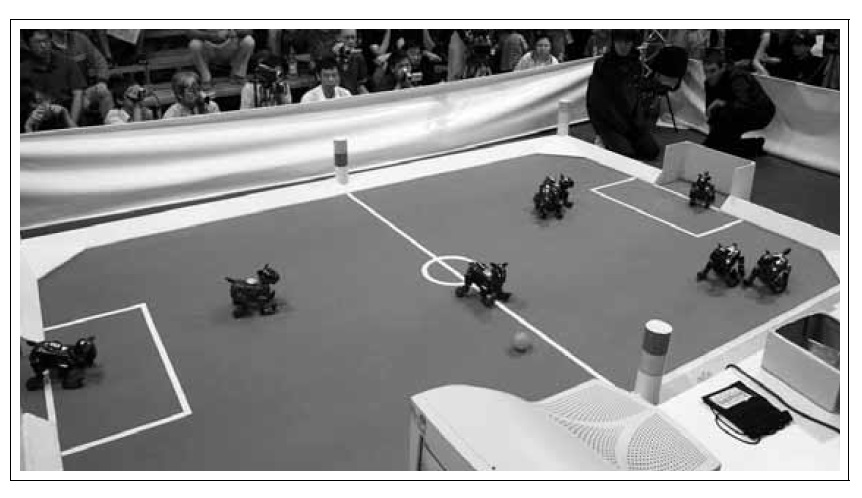
\includegraphics[width=1\linewidth]{77orig}}
	\caption{ (  Рис. 7.7 Роботы AIBO на футбольном поле RoboCup. По углам поля и на центральных линиях расположены шесть ориентиров. )}
	\label{fig:77orig}
\end{figure}

\textbf{7.4.4 Физическая реализация}\\

Проиллюстрируем алгоритм EKF на примере локализации четвероногого шагающего робота AIBO на футбольном поле соревнований RoboCup. В данном случае, робот выполняет локализацию на основе шести маркеров разных цветов, размещённых вокруг поля (см. Рис. 7.7). Также, как в алгоритме EKF, приведённом в Таблице 7.2, управление перемещением $u_t = (v_t\, \omega_t)^T$ моделируется поступательной и вращательной скоростью, а наблюдения $z_t = (r_t\, \phi_t\, s_t)^T$ содержат значения относительного расстояния и направления на маркер. 
Для простоты допустим, что робот обнаруживает только один маркер в один момент времени.\\

\textbf{Этап экстраполяции (Строки 3–7)} На Рис. 7.8 показан этап экстраполяции алгоритма локализации EKF. На нем изображена неопределённость экстраполяции, появившаяся в результате различных параметров шумов движения, $\alpha_1-\alpha_4$, используемых в строке 5 алгоритма. Параметры $\alpha_2$ и $\alpha_3$ установлены в значение 5\% во всех визуализациях.
Основные параметры зашумления поступательного и вращательного движения $\alpha_1$ и $\alpha_4$ варьируются между $\langle10\%, 10\%\rangle, \langle30\%, 10\%\rangle, \langle10\%, 30\%\rangle, и \langle30\%, 30\%\rangle$ (от верхнего левого до нижнего правого на Рис. 7.8). На каждом графике робот выполняет действие управления $u_t = \langle10 \text{см/сек}, 5^\circ\text{/сек}\rangle$ на 9 сек, что приводит к перемещению по дуге длиной 90 см и повороту на $45^\circ$. Оценка предыдущего местоположения робота отображается эллипсом с центром в точке математического ожидания $\mu_{t-1} = \langle80, 100, 0\rangle$.

Алгоритмом EKF вычисляется прогнозируемое математическое ожидание $\bar{\mu}_t$ сдвигом предыдущей оценки при условии идеального движения (строка 6). Соответствующий эллипс неопределённости $\bar{\varSigma}_t$, состоит из двух компонентов. Одна оценивает неопределённость начального местоположения, другая – неопределённость, вызванную шумами движения (строка 7). 

\begin{figure}[H]
	\center{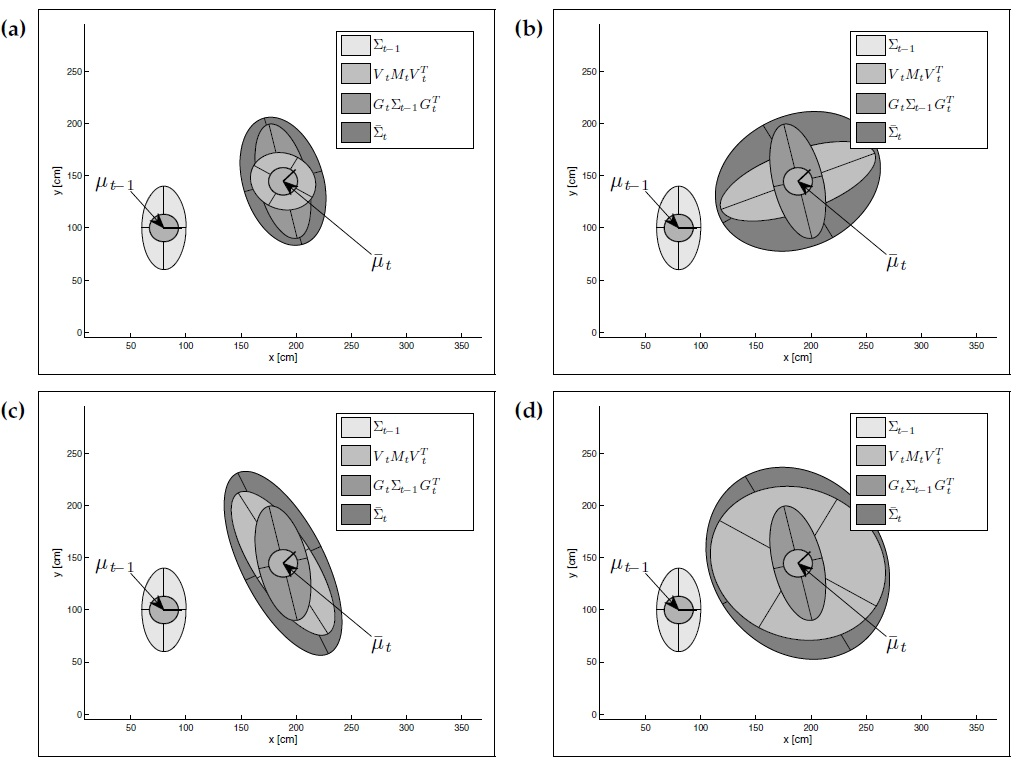
\includegraphics[width=0.95\linewidth]{78orig}}
	\caption{ (  Рис. 7.8 Такт экстраполяции алгоритма EKF. Схемы были сгенерированы с различными параметрами шумов движения. Начальная оценка робота показана эллипсом с центром в $\mu_{t-1}$. После движения по пути длиной 90 см и поворота на 45 градусов влево, прогнозируемое положение имеет центр в $\bar{\mu}_t$. На схеме (a) шум движения относительно мал как для поступательного движения, так и для вращательного. На других схемах показаны: (b) большое зашумление поступательного движения, (c) большое зашумление вращательного движения и (d) большое зашумление поступательного и вращательного движения. )}
	\label{fig:78orig}
\end{figure}

Первый компонент $G_t\varSigma_{t-1}G_t^T$ игнорирует шумы движения и проектирует предыдущую неопределённость $\varSigma_{t-1}$ с помощью линейной аппроксимации функции движения. Из выражений (7.8) и (7.9) вспомним, что линейная аппроксимация представлена матрицей $G_t$, которая является якобианом функции движения относительно предыдущего положения робота.

Результирующие эллипсы зашумления идентичны на всех четырёх схемах, поскольку шум движения не учитывается. Неопределённость шума движения моделируется вторым компонентом $\bar{\varSigma}_t$, заданным в виде $V_t\, M_t\, V_t^T$ (строка 7). Матрица $M_t$ представляет шум движения в пространстве сигналов управления (строка 5). Эта матрица шумов движения проектируется в пространство состояний умножением на $V_t$, который является якобианом функции управления движения (строка 4). Как видно, результирующий эллипс отображает большую ошибку поступательной скорости ($\alpha_1 = 30\%$) в виде большой неопределённости вдоль направления движения (правые графики на Рис. 7.8).
Большая ошибка скорости вращения ($\alpha_4 = 30\%$) приводит к большой неопределённости перпендикулярно направлению движения (нижние графики на Рис. 7.8). Общая неопределённость прогноза $\bar{\varSigma}_t$ задана сложением двух компонент.

\begin{figure}[H]
	\center{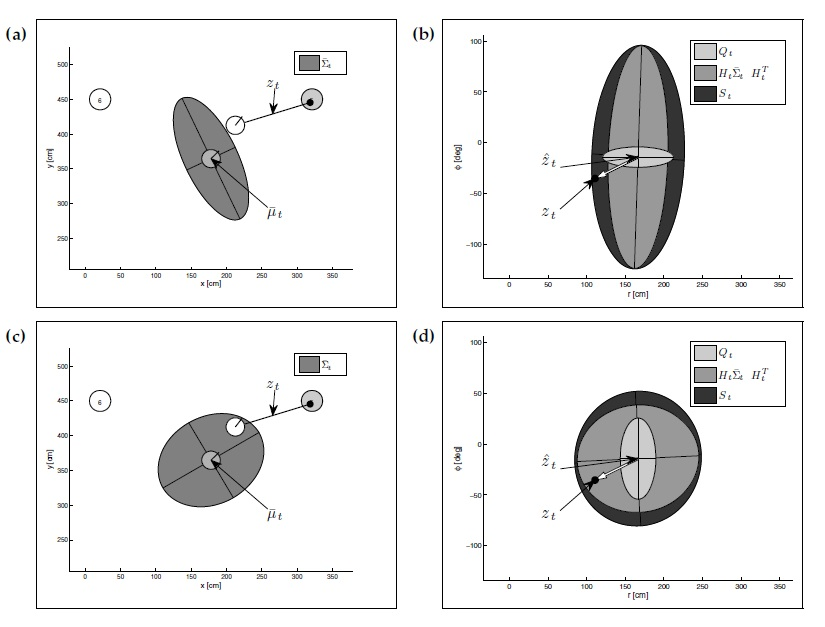
\includegraphics[width=1\linewidth]{79orig}}
	\caption{ (  Рис. 7.9 Экстраполяция измерения. На левом графике показаны два прогнозируемых местоположения робота, а также их эллипсы неопределенности. Настоящий робот и его наблюдения показаны белым кругом и жирной линией, соответственно. На схемах справа показаны результирующие прогнозы измерений. Белыми стрелками показан параметр "innovation" - разница между наблюдаемыми и прогнозируемыми измерениями.)}
	\label{fig:79orig}
\end{figure}

\textbf{Такт коррекции: Прогноз измерения (Строки 8–14).} В первой части такта коррекции алгоритм EKF выполняет прогноз измерения, $\bar{z}_t$, используя прогнозируемое местоположение робота и его неопределённость. На Рис. 7.9 показано прогнозирование измерения. На левых графиках показаны прогнозируемые местоположения робота и их эллипсы неопределённости. Истинное местоположение робота обозначено белым кругом. Теперь допустим, робот наблюдает ориентир впереди справа (показано жирной линией). На схемах справа показаны соответствующие прогнозируемые и текущие измерения в пространстве измерений. Прогнозируемое измерение $\bar{z}_t$ вычисляется из относительного расстояния и угла направления между прогнозируемым математическим ожиданием $\bar{\mu}_t$ и наблюдаемым ориентиром (строка 12).
Неопределённость этого прогноза представлена эллипсом $S_t$. Аналогично прогнозированию состояния, неопределённость возникает из свёртки двух гауссовых функций. Эллипс $Q_t$ представляет неопределённость шума измерений (строка 8), а эллипс $H_t\bar{\varSigma}_tH_t^T$ определяет неопределённость местоположения робота. Неопределённость местоположения робота $\bar{\varSigma}_t$ проектируется на неопределённость наблюдения путём умножения на якобиан функции измерения $H_t$, относящийся к местоположению робота (строка 13). 

\begin{figure}[H]
	\center{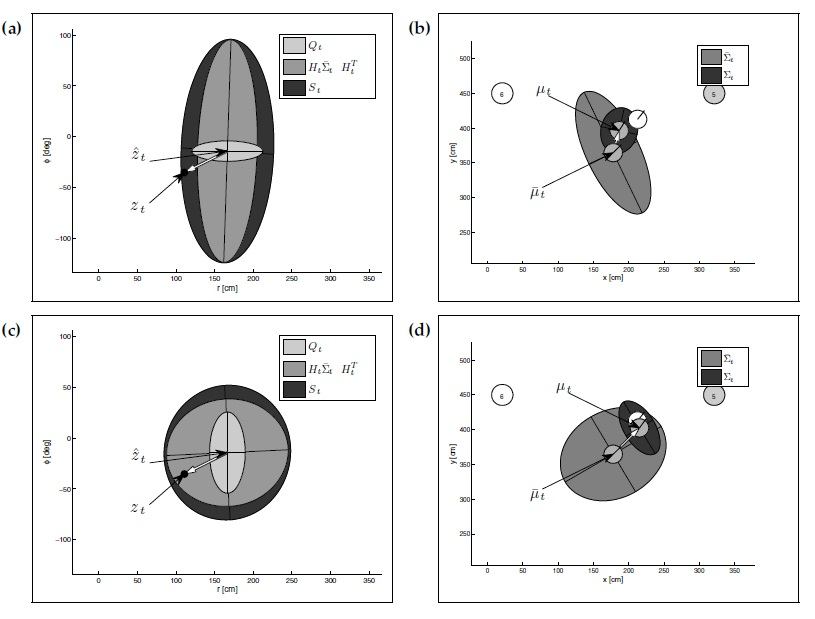
\includegraphics[width=0.9\linewidth]{710orig}}
	\caption{ (  Рис. 7.10 Такт коррекции алгоритма EKF. На графиках слева показаны прогнозы измерения, а на графиках справа – результирующие коррекции, которые обновляют среднюю оценку и уменьшают эллипсы неопределённости положения. )}
	\label{fig:710orig}
\end{figure}


$S_t$, общая неопределенность прогноза измерения, представляет собой сумму этих двух эллипсов (строка 14).\\
MEASUREMENT INNOVATION\\ Белыми стрелками
на графиках показаны так называемые \textit{innovation vector - векторы изменения} $z_t-\bar{z}_t$, представляющие собой просто разницу между наблюдаемым и прогнозируемым измерением. Эти векторы играет ключевую роль в последующем такте обновления. Он также предоставляет правдоподобие измерения $z_t$, которое задано правдоподобием векторов изменений для гауссовой функции с нулевым математическим ожиданием с ковариацией $S_t$ (строка 21). Таким образом, чем короче «короткий»  (в смысле расстояния Махаланобиса) вектор изменений, тем более вероятно измерение.\\

\textbf{Такт коррекции: Обновление оценки (строки 15–21)} Такт коррекции алгоритма локализации EKF показан на Рис. 7.10 и выполняет обновление оценки местоположения на основе вектора изменения и неопределённости прогноза измерения. Для удобства на графиках слева снова показана гипотеза измерения. На графиках справа показаны результирующие коррекции оценок местоположений, что показано белыми стрелками. Эти векторы коррекции вычисляются масштабной проекцией вектора изменений измерений (белые стрелки на левых графиках) в пространство состояний (строка 16). Это проектирование и масштабирование выполняется с помощью матрицы усиления Калмана $K_t$, вычисленной в строке 15. Очевидно, изменения измерения выражают смещение между прогнозируемым и наблюдаемым измерением. Это смещение затем проектируется в пространство состояний и используется для сдвига оценки местоположения в направлении уменьшения изменения.  Усиление Калмана дополнительно масштабирует вектор изменений, таким образом, учитывая неопределённость в прогнозе измерения. Чем более точное измерение, тем выше усиление Калмана, и тем сильнее результирующая коррекция местоположения. Эллипс неопределённости оценки местоположения обновляется в соответствии с похожей логикой (строка 17).

\begin{figure}[H]
	\center{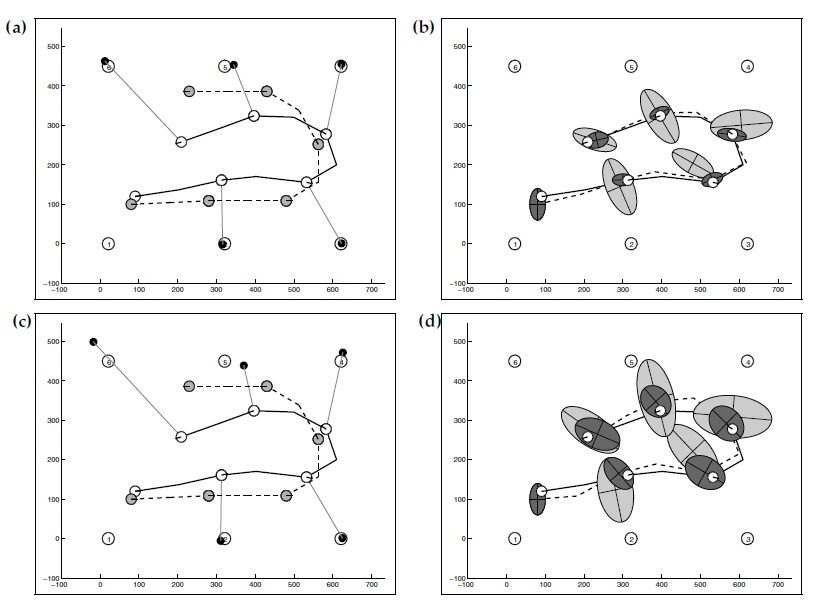
\includegraphics[width=0.85\linewidth]{711orig}}
	\caption{ (  Рис. 7.11 Локализация на основе EKF с точным (верхний ряд) и неточным (нижний ряд) датчиками обнаружения ориентиров. Пунктирными линиями на левом графике показаны траектории робота, оценённые на основе управления движением. Сплошные линии обозначают реальное движение робота на основе этих управляющих воздействий. Обнаруженные в пяти точках ориентиры указаны тонкими линиями. Пунктирные линии на правых графиках демонстрируют скорректированные траектории робота, а также неопределённость до (светло-серый цвет, $\bar{\varSigma}_t$) и после (темно-серый цвет, $\varSigma_t$) учёта обнаружения ориентира.)}
	\label{fig:711orig}
\end{figure}

\textbf{Пример последовательности.} На Рис. 7.11 показаны две последовательности обновлений EKF, используя различные неопределённости наблюдения. На левых графиках показаны траектории робота согласно управлению движением (пунктирные линии) и результирующие реальные траектории (жирные линии). Обнаружения ориентиров показаны тонкими линиями, измерения на верхних графиках менее зашумлены. Пунктирными линиями на правых графиках показаны пути, вычисленные после оценки алгоритмом локализации EKF. Как и ожидалось, меньшая неопределённость измерения в верхнем ряду ведёт к меньшему размеру эллипсов неопределённости и меньшим ошибкам оценки.\\

\textbf{7.5 Оценка соответствия}\\

\textbf{7.5.1 Локализация EKF с неизвестным соответствием}\\

Локализация с помощью EKF, обсуждаемая до текущего момента, применима только когда соответствия ориентиров могут быть определены с абсолютной точностью. На практике такое происходит редко, поэтому в большинстве реализаций определение ориентира происходит во время локализации. В ходе изложения мы столкнёмся с рядом стратегий для решения проблемы соответствия. Самая простая из них известна как соответствие максимального правдоподобия.\\
СООТВЕТСТВИЕ МАКСИМАЛЬНОГО ПРАВДОПОДОБИЯ\\
Сначала определяется самое вероятное значение переменной соответствия, а затем это значение принимается как эталонное. 

Методы максимального правдоподобия неустойчивы, если для переменной соответствия имеется множество равновероятных гипотез. Однако, часто можно спроектировать систему таким образом, чтобы этого избежать. Для предотвращения ошибочной ассоциации данных имеется два метода. Во-первых, можно выбирать достаточно уникальные и достаточно далеко расположенные друг от друга ориентиры, чтобы перепутать их было затруднительно. Во-вторых, гарантировать малую неопределённость положения робота. К сожалению, эти два метода несколько противоречат друг другу, а нахождение верного разбиения ориентиров в окружающей среде сродни искусству. 

В любом случае, методы максимального правдоподобия имеют огромное практическое значение. В Таблице 7.3 приведён алгоритм локализации на основе EKF с оценкой максимального правдоподобия для соответствия. Обновление движения в строках со 2 по 7 идентично таковому в Таблице 7.2. Ключевая разница заключается в обновлении измерения: для каждого измерения сначала вычисляется количество элементов, позволяющее определить наиболее вероятное соответствие для всех $k$ ориентиров карты (строки с 10 до 15). Переменная соответствия $j(i)$ выбирается в строке 16 с помощью максимизации правдоподобия измерения $z^i_t$ заданной для каждого возможного ориентира $m_k$ на карте. Заметим, что эта функция правдоподобия идентична функции, используемой алгоритмом EKF для известного соответствия. Обновление EKF в строках 18 и 19 учитывает только наиболее вероятные соответствия.

Заметим, что алгоритм в Таблице 7.3 не слишком эффективен. Его можно улучшить более вдумчивым выбором ориентиров в строке 10. В большинстве ситуаций робот способен одновременно воспринимать только небольшое количество ориентиров в непосредственной близости, но с помощью простых тестов можно отбросить множество ориентиров с малой вероятностью на карте. \\

\textbf{7.5.2 Математический вывод ассоциации данных с помощью ML} \\

Оценочная функция максимального правдоподобия определяет соответствие, которое максимизирует правдоподобие данных.

\begin{table}[H]
\begin{center}
\begin{tabular}{|l|}
\hline
{}\\
1: Algorithm EKF\_localization$(\mu_{t-1},\varSigma_{t-1},u_t,z_t,m):$ \\
2:\hspace{5mm}$\theta=\mu_{t-1,\theta}$\\
3:\hspace{5mm}
\begin{minipage}{0.2\textwidth}
\begin{equation*}
G_t=
\left(\begin{array}{ccc}
1&0&-\frac{\upsilon_t}{\omega_t}\cos\theta+\frac{\upsilon_t}{\omega_t}\cos(\theta+\omega_t\varDelta t)\\
0&1&-\frac{\upsilon_t}{\omega_t}\sin\theta+\frac{\upsilon_t}{\omega_t}\sin(\theta+\omega_t\varDelta t)\\
0&0&1\\
\end{array}\right)
\end{equation*}
\end{minipage}\\
4:\hspace{5mm}
\begin{minipage}{0.2\textwidth}
\begin{equation*}
V_t=
\left(\begin{array}{cc}
\frac{-\sin\theta+\sin(\theta+\omega_t\varDelta t)}{\omega_t}&\frac{\upsilon_t(\sin\theta-\sin(\theta+\omega_t\varDelta t))}{\omega_t^2}+\frac{\upsilon_t\cos(\theta+\omega_t\varDelta t)\varDelta t}{\omega_t}\\
\frac{\cos\theta-\cos(\theta+\omega_t\varDelta t)}{\omega_t}&-\frac{\upsilon_t(\cos\theta-\cos(\theta+\omega_t\varDelta t))}{\omega_t^2}+\frac{\upsilon_t\sin(\theta+\omega_t\varDelta t)\varDelta t}{\omega_t}\\
0&\varDelta t\\
\end{array}\right)
\end{equation*}
\end{minipage}\\
5:\hspace{5mm}
\begin{minipage}{0.2\textwidth}
\begin{equation*}
M_t=
\left(\begin{array}{cc}
\alpha_1\upsilon_t^2+\alpha_2\omega_t^2&0\\
0&\alpha_3\upsilon_t^2+\alpha_4\omega_t^2\\
\end{array}\right)
\end{equation*}
\end{minipage}\\
6:\hspace{5mm}
\begin{minipage}{0.2\textwidth}
\begin{equation*}
\bar{\mu}_t=\mu_{t-1}+
\left(\begin{array}{c}
-\frac{\upsilon_t}{\omega_t}\sin\theta+\frac{\upsilon_t}{\omega_t}\sin(\theta+\omega_t\varDelta t)\\
\frac{\upsilon_t}{\omega_t}\cos\theta-\frac{\upsilon_t}{\omega_t}\cos(\theta+\omega_t\varDelta t)\\
\omega_t\varDelta t\\
\end{array}\right)
\end{equation*}
\end{minipage}\\
7:\hspace{5mm}$\bar{\varSigma}_t=G_t\varSigma_{t-1}G_t^T+V_tM_tV_t^T$\\
8:\hspace{5mm}
\begin{minipage}{0.2\textwidth}
\begin{equation*}
Q_t=
\left(\begin{array}{ccc}
\sigma^2_r&0&0\\
0&\sigma^2_\phi&0\\
0&0&\sigma^2_s\\
\end{array}\right)
\end{equation*}
\end{minipage}\\
9:\hspace{6mm}$\textit{for all observed features}\,z_t^i=(r_t^i\,\phi_t^i\,s_t^i)^T\textit{do}$\\
10:\hspace{10mm}$\textit{for all landmarks} k \textit{in the map} m \textit{do}$\\
11:\hspace{15mm}$q=(m_{k,x}-\bar{\mu}_{t,x})^2+(m_{k,y}-\bar{\mu}_{t,y})^2$\\
12:\hspace{15mm}
\begin{minipage}{0.2\textwidth}
\begin{equation*}
\hat{z}_t^k=
\left(\begin{array}{c}
\sqrt{q}\\
\text{atan}2(m_{k,y}-\bar{\mu}_{t,y},m_{k,x}-\bar{\mu}_{t,x})-\bar{\mu}_{t,\theta}\\
m_{k,s}\\
\end{array}\right)
\end{equation*}
\end{minipage}\\
13:\hspace{15mm}
\begin{minipage}{0.2\textwidth}
\begin{equation*}
H_t^k=
\left(\begin{array}{ccc}
-\frac{m_{k,x}-\bar{\mu}_{t,x}}{\sqrt{q}}&-\frac{m_{k,y}-\bar{\mu}_{t,y}}{\sqrt{q}}&0\\
\frac{m_{k,y}-\bar{\mu}_{t,y}}{q}&-\frac{m_{k,x}-\bar{\mu}_{t,x}}{q}&-1\\
0&0&0\\
\end{array}\right)
\end{equation*}
\end{minipage}\\
14:\hspace{15mm}$S_t^k=H_t^k\bar{\varSigma}_t[H_t^k]^T+Q_t$\\
15:\hspace{10mm}$\textit{endfor}$\\
16:\hspace{10mm}$j(i)=\underset{k}{\text{argmax}}\,\,\det(2\pi S_t^k)^{-\frac{1}{2}}\exp\{-\frac{1}{2}(z_t^i-\hat{z}_t^k)^T[S_t^k]^{-1}(z_t^i-\hat{z}_t^k)\}$\\
17:\hspace{10mm}$K_t^i=\bar{\varSigma}_t[H_t^{j(i)}]^T[S_t^{j(i)}]^{-1}$\\
18:\hspace{10mm}$\bar{\mu}_t=\bar{\mu}_t+K_t^i(z_t^i-\hat{z}_t^{j(i)})$\\
19:\hspace{10mm}$\bar{\varSigma}_t=(I-K_t^i\,H_t^{j(i)})\bar{\varSigma}_t$\\
20:\hspace{4mm}$\textit{endfor}$\\
21:\hspace{4mm}$\mu_t=\bar{\mu}_t$\\
22:\hspace{4mm}$\varSigma_t=\bar{\varSigma}_t$\\
23:\hspace{4mm}$\textit{return}\,\mu_t,\varSigma_t$\\
{}\\
\hline
\end{tabular}
\caption{(Таблица 7.3 Алгоритм локализации на основе обобщённого фильтра Калмана (EKF) с неизвестным соответствием. Соответствия $j(i)$ оцениваются с помощью алгоритма максимального правдоподобия.)}
\end{center}
\end{table}

(7.22) 
$$\hat{c}_t=\underset{c_t}{\text{argmax}}\,p(z_t|c_{1:t},m,z_{1:t-1},u_{1:t})$$

Здесь $c_t$ вектор соответствия в момент времени $t$. Как и прежде, вектор $z_t = \{z_t^1, z_t^2, . . .\}$ – это вектор измерений, содержащий список признаков или ориентиров $z_t^i$, наблюдаемых в момент времени $t$.

Оператор argmax в выражении (7.22) выбирает вектор соответствия $\hat{c}_t$, который максимизирует правдоподобие измерения. Заметим, что это выражение основано на предыдущих соответствиях $c_{1:t-1}$. Хотя они были оценены во время предыдущих шагов обновления, в методе максимального правдоподобия считается, что они всегда верны. Это имеет два важных последствия. Во-первых, это даёт возможность инкрементного обновления фильтра. Но, вместе с этим, фильтр становится неустойчивым, его значения отклоняются при ошибочных оценках соответствия. 
 
Даже при условии известного предыдущего соответствия, присутствует экспоненциальное множество членов максимизации (7.22). При большом количестве обнаруженных ориентиров во время одного измерения число возможных соответствий может стать чрезмерно большим для практического использования. Наиболее часто используемый метод, позволяющий избежать экспоненциальной сложности, выполняет максимизацию для каждого индивидуального признака $z_t^i$ в векторе измерений $z_t$. Мы уже вывели функцию правдоподобия для отдельных признаков в выводе алгоритма локализации на основе EKF с известными соответствиями. Следуя уравнениям с (7.17) до (7.20), соответствие каждого признака вычисляется как:\\

(7.23) 
\begin{equation*}
\begin{split}
\hat{c}_t^i&=\underset{c_t^i}{\text{argmax}}\,p(z_t^i|c_{1:t},m,z_{1:t-1},u_{1:t})\\
&\approx\underset{c_t^i}{\text{argmax}}\,\mathcal{N}(z_t^i;h(\bar{\mu}_t,c_t^i,m),H_t\bar{\varSigma}_tH_t^T+Q_t)
\end{split}
\end{equation*}

Это вычисление выполняется в строке 16 в Таблице 7.3. Эта покомпонентная оптимизация «оправдана» только если известно, что отдельные векторы признаков условно независимы. Это допущение обычно делается для удобства вычисления. При таком допущении максимизируемый член в выражении (7.22) выражен произведением  членов с несовместными параметрами оптимизации. Максимум произведения достигается, когда каждый множитель максимален, как определено в (7.23). При использовании этой ассоциации данных максимального правдоподобия, правильность алгоритма напрямую следует из правильности алгоритма локализации на основе EKF с известными соответствиями.\\

\textbf{7.6 Отслеживание нескольких гипотез}\\

Существует несколько обобщений базового EKF, позволяющих приспособить его для ситуаций, при которых верная ассоциация данных не может быть определена с удовлетворительной надёжностью. Некоторые из этих методов будут обсуждаться позже в книге, поэтому сейчас остановимся на них лишь кратко.

Классический метод, который позволяет обойти ограничения ассоциации данных, это фильтр с\textit{отслеживания нескольких гипотез} или MHT. Фильтр MHT способен представлять оценку с помощью нескольких гауссовых функций. В нём апостериорное распределение представлено в виде смеси\\

(7.24)
$$bel(x_t)=\frac{1}{\sum_l\psi_{t,l}}\sum_l\psi_{t,l}\det(2\pi\varSigma_{t,l})^{-\frac{1}{2}}\exp\left\lbrace -\frac{1}{2}(x_t-\mu_{t,l})^T\varSigma_{t,l}^{-1}(x_t-\mu_{t,l})\right\rbrace $$

Здесь $l$ – индекс компонента смеси. Каждый такой компонент или «след» на жаргоне MHT, представляет собой гауссову функцию с математическим ожиданием $\mu_{t,l}$ и ковариацией $\varSigma_{t,l}$.\\
ВЕС СМЕСИ\\ Скаляр $\psi_{t,l}\geq0$ это \textit{вес смеси}. Он определяет вес $l$-го компонента смеси в апостериорном распределении. Поскольку апостериорное распределение нормализовано с помощью $\varSigma_l\psi_{t,l}$, каждая величина $\psi_{t,l}$ – это относительный вес, и вклад $l$-го компонента смеси зависит от величины всех прочих весов смеси.

Как будет показано ниже при описании алгоритма MHT, каждый компонент смеси основан на уникальном решении последовательности  ассоциации данных. Поэтому, имеет смысл записать $c_{t,l}$ для вектора ассоциации данных, связанного с $l$-им следом, а $c_{1:t,l}$ – для всех прошлых и настоящих ассоциаций данных, связанных с $l$-м компонентом смеси. В такой записи можно считать смесь компонентов в виде содействующих функций локальных оценок, основанных на уникальной последовательности ассоциации данных:\\

(7.25)
$$bel_l(x_t)=p(x_t|z_{1:t},u_{1:t},c_{1:t,l})$$

Здесь $c_{1:t,l}={c_{1,l}, c_{2,l}, . . . , c_{t,l}}$ определяют последовательность векторов соответствия, связанных с $l$-м следом.

Прежде чем описывать MHT,  обсудим полностью неразрешимый алгоритм, из которого выводится MHT. Это алгоритм полной реализации теоремы Байеса для EKF с неизвестной ассоциацией данных.
Он удивительно прост: Вместо того, чтобы выбирать наиболее вероятный вектор ассоциации данных, наш вымышленный алгоритм сохраняет их все. А именно, пусть для момента времени $t$ каждая смесь разделяется на множество новых смесей, каждая из которых основана на уникальном векторе соответствия $c_t$. Пусть $m$ будет индексом одного из новых гауссовых распределений, а $l$ – индексом, для соответствия $c_{t,l}$, из которого это новое распределение было выведено. Вес этой новой смеси затем устанавливается как \\

(7.26)
$$\psi_{t,m}=\psi_{t,l}\,p(z_t|c_{1:t-1,l},c_{t,m},z_{1:t-1},u_{1:t})$$

Это произведение веса смеси $\psi_{t,l}$ из которой был выведен новый компонент и правдоподобие измерения $z_t$ при определённом векторе соответствия, приводящему к образованию нового компонента смеси. Другими словами, можно вычислить соответствие латентной переменной и апостериорное правдоподобие того, что компонент смеси верен. Способ вычисления правдоподобия измерения $p(z_t | c_{1:t-1,l}, c_{t,m}, z_{1:t-1}, u_{1:t})$ уже известен из выражения (7.26). Это просто правдоподобие измерения, вычисленное в строке 21 алгоритма локализации на основе EKF для известных ассоциаций данных (Таблица 7.2). Отсюда, можно последовательно вычислить веса смеси каждого нового компонента. Единственным недостатком этого алгоритма является факт экспоненциального увеличения со временем количества компонентов смеси, или следов. 

Алгоритм MHT является приближением описанного метода с сохранением небольшого количества компонентов смеси.\\
ПРУНИНГ\\
Этот процесс называется прунинг (pruning - отсечение). Во время прунинга уничтожается каждый компонент с относительным весом смеси \\

(7.27)
$$\frac{\psi_{t,l}}{\sum_m \psi_{t,m}}$$

менее порогового значения $\psi_{min}$. Легко увидеть, что количество компонентов смеси всегда будет максимум $\psi_{min}^{-1}$. Таким образом, в MHT сохраняется компактный вид апостериорного распределения, которое можно эффективно обновлять. Приближение достигается сохранением очень малого числа гауссовых функций, но на практике и количество вероятных местонахождений робота обычно очень невелико. 

Пропустим формальное описание алгоритма MHT, предоставив читателю возможность ознакомиться с большим числом подобных алгоритмов, описанных в книге. 
Стоит отметить, что при реализации алгоритмов MHT полезно заранее определять стратегии идентификации следов с низким правдоподобием.\\

\textbf{7.7 Локализация на основе UKF }\\

UKF локализация – это алгоритм локализации робота на основе признаков, использующий unscented Kalman filter. Как описано в подразделе 3.4,  для линеаризации моделей движения и измерения в UKF используется unscented преобразование. Вместо вычисления производных этих моделей, unscented преобразование представляет гауссианы с помощью сигма-точек и передаёт их в модели. В Таблице 7.4 приводится алгоритм UKF локализации робота на основе ориентиров.
Предполагается, что в наблюдении $z_t$ содержится единственное наблюдение ориентира, а идентификатор этого ориентира известен заранее.\\

\textbf{7.7.1 Математический вывод UKF локализации}\\

Главным образом, локализация и общий алгоритм UKF, приведённый в Таблице 3.4, различаются способом прогнозирования и измерения шумов.
Напомним, что UKF из Таблице 3.4 основан на допущении аддитивности прогноза и измерения. В силу этого, возможно вычислить зашумление простым суммированием $R_t$ и $Q_t$ и прогнозируемой неопределённости состояния и измерения, соответственно (строки 5 и 9 в Таблице 3.4).\\

\begin{table}[H]
\begin{center}
\begin{tabular}{|l|}
\hline
{}\\
1: Algorithm UKF\_localization$(\mu_{t-1},\varSigma_{t-1},u_t,z_t,m):$ \\
\hspace{3mm}$\textit{Generate augmented mean and covariance}$\\
2:\hspace{5mm}
\begin{minipage}{0.2\textwidth}
\begin{equation*}
M_t=
\left(\begin{array}{cc}
\alpha_1\upsilon_t^2+\alpha_2\omega_t^2&0\\
0&\alpha_3\upsilon_t^2+\alpha_4\omega_t^2\\
\end{array}\right)
\end{equation*}
\end{minipage}\\
3:\hspace{5mm}
\begin{minipage}{0.2\textwidth}
\begin{equation*}
Q_t=
\left(\begin{array}{cc}
\sigma^2_r&0\\
0&\sigma^2_\phi\\
\end{array}\right)
\end{equation*}
\end{minipage}\\
4:\hspace{5mm}
$\mu_{t-1}^a=(\mu_{t-1}^T\,\,(0\,\,0)^T\,\,(0\,\,0)^T)^T$\\
5:\hspace{5mm}
\begin{minipage}{0.2\textwidth}
\begin{equation*}
\varSigma_{t-1}^a=
\left(\begin{array}{ccc}
\varSigma_{t-1}&0&0\\
0&M_t&0\\
0&0&Q_t\\
\end{array}\right)
\end{equation*}
\end{minipage}\\
\hspace{3mm}$\textit{Генерация сигма-точек}$\\
6:\hspace{5mm}$\mathcal{X}_{t-1}^a=(\mu_{t-1}^a\,\,\,\,\mu_{t-1}^a+\gamma\sqrt{\varSigma_{t-1}^a}\,\,\,\,\mu_{t-1}^a-\gamma\sqrt{\varSigma_{t-1}^a})$\\
\hspace{3mm}$\textit{Пропускание сигма-точек через модель движения и вычисление статистик гауссовых функций}$\\
7:\hspace{5mm}$\bar{\mathcal{X}}_t^x=g(u_t+\mathcal{X}_t^u,\mathcal{X}_{t-1}^x)$\\
8:\hspace{5mm}$\bar{\mu}_t=\sum_{i=0}^{2L}w_i^{(m)}\bar{\mathcal{X}}_{i,t}^x$\\
9:\hspace{5mm}$\bar{\varSigma}_t=\sum_{i=0}^{2L}w_i^{(c)}(\bar{\mathcal{X}}_{i,t}^x-\bar{\mu}_t)(\bar{\mathcal{X}}_{i,t}^x-\bar{\mu}_t)^T$\\
\hspace{3mm}$\textit{Прогнозирование производных в сигма-точках и вычисление статистик гауссовых функций}$\\
10:\hspace{4mm}$\bar{Z}_t=h(\bar{\mathcal{X}}_t^x)+\mathcal{X}_t^z$\\
11:\hspace{4mm}$\hat{z}_t=\sum_{i=0}^{2L}w_i^{(m)}\bar{Z}_{i,t}$\\
12:\hspace{4mm}$S_t=\sum_{i=0}^{2L}w_i^{(c)}(\bar{Z}_{i,t}-\hat{z}_t)(\bar{Z}_{i,t}-\hat{z}_t)^T$\\
13:\hspace{4mm}$\varSigma_t^{x,z}=\sum_{i=0}^{2L}w_i^{(c)}(\bar{\mathcal{X}}_{i,t}^x-\bar{\mu}_t)(\bar{Z}_{i,t}-\hat{z}_t)^T$\\
\hspace{3mm}$\textit{Обновление значений среднего и ковариации}$\\
14:\hspace{4mm}$K_t=\varSigma_t^{x,z}S_t^{-1}$\\
15:\hspace{4mm}$\mu_t=\bar{\mu}_t+K_t(z_t-\hat{z}_t)$\\
16:\hspace{4mm}$\varSigma_t=\bar{\varSigma}_t-K_t S_t K_t^T$\\
17:\hspace{4mm}$p_{z_t}=\det(2\pi S_t)^{-\frac{1}{2}}\exp\{-\frac{1}{2}(z_t-\hat{z}_t)^T\,S_t^{-1}(z_t-\hat{z}_t)\}$\\
18:\hspace{4mm}$\textit{return}\,\mu_t,\varSigma_t,p_{z_t}$\\
{}\\
\hline
\end{tabular}
\caption{(Таблица 7.4 Алгоритм локализации unscented Kalman filter (UKF), сформулированный для карты на основе признаков и робота, оснащённого датчиками измерения расстояния и угла направления. В этой версии обрабатывается единичные наблюдения ориентиров и подразумевается знание точного соответствия. Величина $L$ – размерность дополненного вектора состояний, заданного суммой размерностей состояния, управления и измерения. )}
\end{center}
\end{table}

\textbf {Алгоритм UKF\_localization} реализует другой, более точный метод учёта влияния шумов на процесс оценки. Ключевым действием является дополнение состояния с помощью компонент, отображающих шумы управления и измерения. Размерность $L$ дополненного состояния задана суммой размерности состояния, управления и измерения, которые, в данном случае, равны $3 + 2 + 2 = 7$ (для простоты сигнатура признака измерения  игнорируется). Поскольку в расчёт принят гауссовый шум с нулевым математическим ожиданием, математическое ожидание $\mu_{t-1}^a$ оценки дополненного состояния задано средним оценки местоположения $\mu_{t-1}$ и нулевыми векторами шумов управления и измерения (строка 4).
Ковариация оценки дополненного состояния $\varSigma_{t-1}^a$, заданная комбинацией ковариаций местоположения $\varSigma_{t-1}$, шумов управления $M_t$, и шумов измерения $Q_t$, вычисляется в строке 5.

Отображение оценки дополненного состояния в виде сигма-точек генерируется в строке 6, используя выражение (3.66) для unscented преобразования. В этом примере $\mathcal{X}_{t-1}^a$ содержит $2L + 1 = 15$ сигма-точек, в каждой из которых содержатся компоненты в пространствах состояния, управления и измерения.

(7.28)
\begin{minipage}{0.2\textwidth}\begin{equation*}
\mathcal{X}_{t-1}^a=
\left(\begin{array}{c}
{\mathcal{X}_{t-1}^x}^T\\
{\mathcal{X}_t^u}^T\\
{\mathcal{X}_t^z}^T
\end{array}\right)
\end{equation*}
\end{minipage}\\

Выберем смешанное представление индексов времени, чтобы убедиться, что $\mathcal{X}_{t-1}^x$ относится к $x_{t-1}$, a компоненты управления и измерения - к $u_t$ и $z_t$, соответственно.

Компоненты местоположения $\mathcal{X}_{t-1}^x$ этих сигма-точек затем передаются в модель движения на основе скорости $g$, определённую уравнением (5.9). В строке 7 выполняется такт экстраполяции применением модели движения из уравнения (5.13), используя управляющее воздействие $u_t$ с добавочным компонентом зашумления управления $\mathcal{X}_{i,t}^u$ для каждой сигма-точки:

(7.29)
\begin{minipage}{0.2\textwidth}\begin{equation*}
\bar{\mathcal{X}}_{i,t}^x=\mathcal{X}_{i,t-1}^x+
\left(\begin{array}{c}
-\frac{\upsilon_{i,t}}{\omega_{i,t}}\sin\theta_{i,t-1}+\frac{\upsilon_{i,t}}{\omega_{i,t}}\sin(\theta_{i,t-1}+\omega_{i,t}\varDelta t)\\
\frac{\upsilon_{i,t}}{\omega_{i,t}}\cos\theta_{i,t-1}-\frac{\upsilon_{i,t}}{\omega_{i,t}}\cos(\theta_{i,t-1}+\omega_{i,t}\varDelta t)\\
\omega_{i,t}\varDelta t\\
\end{array}\right)
\end{equation*}
\end{minipage}

где

(7.30)
$$\upsilon_{i,t}=\upsilon_t+\mathcal{X}_{i,t}^{u[\upsilon]}$$

(7.31)
$$\omega_{i,t}=\omega_t+\mathcal{X}_{i,t}^{u[\omega]}$$

(7.32)
$$\theta_{i,t-1}=\mathcal{X}_{i,t-1}^{x[\theta]}$$

сгенерированных из управления $u_t = (\upsilon_t\,\, \omega_t)^T$ и отдельных компонент сигма-точек. Допустим, $\mathcal{X}_{i,t}^{u[\upsilon]}$ отображает поступательную скорость $\upsilon_t$ для $i$-й сигма-точки. Прогнозируемые сигма-точки, $\bar{\mathcal{X}}_t^x$, таким образом, представляют местоположения робота, которые складываются из различных комбинация предыдущих управляющих воздействий и измерений. 

В строках 8 и 9 вычисляется математическое ожидание и ковариация прогнозируемого местоположения робота, используя метод unscented преобразования. В строке 9 не требуется добавления компонента шумов движения, который был необходим в алгоритме из Таблицы 3.4. Это происходит потому, что после дополнения состояния прогнозируемые сигма-точки уже содержат шумы движения. Этот факт, вдобавок, делает ненужным копирование сигма-точек из прогнозируемой гауссовой функции (см. строку 6 в Таблице 3.4).

В строке 10, прогнозируемые сигма-точки используются для генерации сигма-точек измерений на основе модели измерений, определённой выражением (6.40) из подраздела 6.6:

(7.33)
\begin{minipage}{0.2\textwidth}\begin{equation*}
\bar{Z}_{i,t}=
\left(\begin{array}{c}
\sqrt{(m_x-\bar{\mathcal{X}}_{i,t}^{x[x]})^2+(m_y-\bar{\mathcal{X}}_{i,t}^{x[y]})^2}\\	
\text{atan}2(m_y-\bar{\mathcal{X}}_{i,t}^{x[y]},m_x-\bar{\mathcal{X}}_{i,t}^{x[y]}-\bar{\mathcal{X}}_{i,t}^{x[\theta]})\\
\end{array}\right)
+
\left(\begin{array}{c}
\mathcal{X}_{i,t}^{z[r]}\\
\mathcal{X}_{i,t}^{z[\phi]}\\
\end{array}\right)
\end{equation*}
\end{minipage}\\

В данном случае шум измерения считается аддитивным.

Оставшиеся шаги обновления идентичны базовому алгоритму UKF, приведённому в Таблице 3.4. В строках 11 и 12 вычисляются математическое ожидание и ковариация прогнозируемого измерения. Взаимная ковариация между местоположением робота и наблюдением определяется в строке 13. В строках с 14 по 16 обновляется оценка местоположения. Правдоподобие измерения вычисляется из вектора изменения и прогнозируемой неопределённости измерения аналогично алгоритму локализации EKF в Таблице 7.2.\\

\textbf{7.7.2 Иллюстрация}\\

Проиллюстрируем алгоритм локализации UKF, используя те же примеры, которые были применены для алгоритма локализации EKF. Читателю предоставляется самому сравнить следующие рисунки с приведёнными в подразделе  7.4.4.\\

\textbf{Такт экстраполяции (Строки 2–9)} На Рис. 7.12 показан такт экстраполяции UKF для разных параметров шумов движения. Компоненты местоположения$\mathcal{X}_{t-1}^x$ сигма-точек, сгенерированных их предыдущей гипотезы обозначены крестиками, расположенными симметрично вокруг $\mu_{t-1}$. 15 сигма-точек обозначают семь разных местоположений робота, из которых после проекции на плоскость видны только пять.

Две дополнительные точки «сверху» и «снизу» средней сигма-точки отображают различные ориентации направления робота. Дугами показан прогноз движения, выполненный в строке 7. Как можно увидеть, было сгенерировано 11 предположений на основе различных комбинаций предыдущих местоположений и шумов движения. На схемах показано воздействие шумов движения на результат обновления. Среднее $\bar{\mu}_t$ и эллипс неопределённости $\bar{\varSigma}_t$ прогнозируемого местоположения робота генерируется из прогнозируемых сигма-точек.

\begin{figure}[H]
	\center{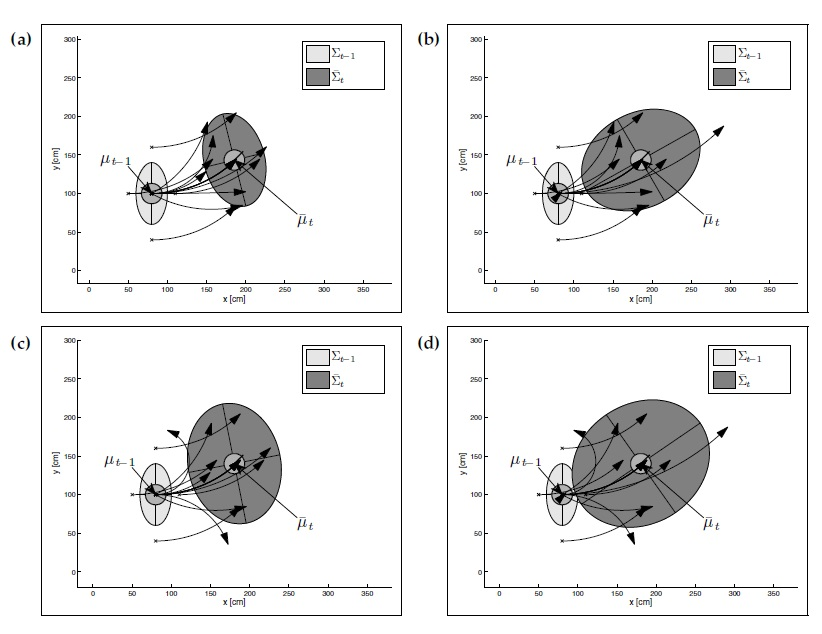
\includegraphics[width=1\linewidth]{712orig}}
	\caption{ (  Рис. 7.12 Этап экстраполяции алгоритма UKF. Графики были сгенерированы с различными параметрами шумов движения. Начальная оценка робота изображена в виде эллипса с центром в $\mu_{t-1}$. Робот движется по дуге длиной 90 см, поворачиваясь на 45 градусов влево. На графике (a) шумы движения относительно малы как для поступательной, так и для вращательной скорости. На других графиках показаны: (b) большие шумы поступательного движения, (c) большие шумы вращательного движения (d) высокие шумы как поступательного, так и вращательного движения. )}
	\label{fig:712orig}
\end{figure}

\textbf{Экстраполяция измерения (Строки 10–12)} В такте экстраполяции измерения прогнозируемые местоположения робота $\bar{\mathcal{X}}_t^x$ используются для генерации сигма-точек измерения $\bar{Z}_t$ (строка 10). Чёрными крестиками на левых графиках Рис. 7.13 показаны локальные сигма-точки, а белые крестики на правых графиках обозначают результирующие сигма-точки измерения. Заметим, что 11 разных сигма-точек положения генерируют 15 разных измерений из-за разных компонентов шумов измерений $\mathcal{X}_t^z$, добавленных в строке 10.
На графиках также показаны математическое ожидание $\hat{z}_t$ и эллипс неопределённости $S_t$ прогнозируемого измерения, которые были вычислены в строках 11 и 12.

\begin{figure}[H]
	\center{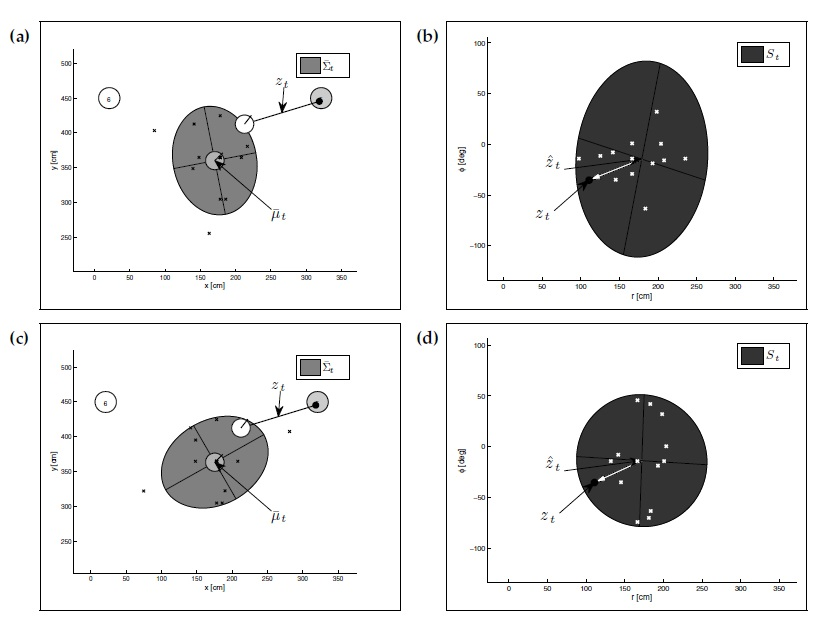
\includegraphics[width=1\linewidth]{713orig}}
	\caption{ (  Рис. 7.13 Прогноз измерения. На графиках слева показаны сигма-точки, прогнозируемые на основе двух обновлений движения, и их результирующие эллипсы неопределённости. Истинное положение робота и наблюдение показаны белым кругом и жирной линией, соответственно. 
	На графиках справа показаны результирующие сигма-точки прогноза измерения. Белыми стрелками показаны векторы изменения, разницы между наблюдаемыми и прогнозируемыми измерениями.
		 )}
	\label{fig:713orig}
\end{figure}

\textbf{Такт коррекции: Обновление оценки (Lines 14–16)} Такт коррекции алгоритма локализации UKF практически идентичен такту коррекции EKF. Вектор изменения и неопределённость прогноза измерения используются для обновления оценки, как показано белой стрелкой на Рис. 7.14.\\

\begin{figure}[H]
	\center{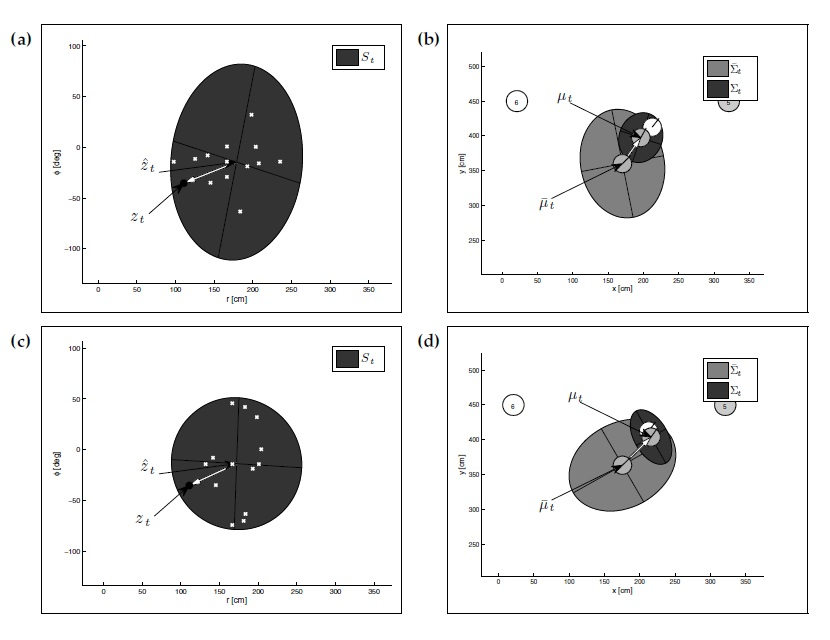
\includegraphics[width=1\linewidth]{714orig}}
	\caption{ (  Рис. 7.14 Такт коррекции алгоритма UKF. На схемах с левой стороны показаны  прогноз измерения, а на схемах справа – результирующие коррекции, позволяющие после обновления значений средней оценки уменьшить эллипсы неопределённости позиции.)}
	\label{fig:714orig}
\end{figure}

\textbf{Пример} На Рис. 7.15 показана последовательность оценок местоположения, сгенерированная многочастичным фильтром (сверху справа), EKF (снизу слева) и UKF (снизу справа). На схеме сверху слева показана траектория робота согласно управлению движением (пунктирная линия) и результирующая истинная траектория (жирная линия). Обнаруженные ориентиры показаны тонкими линиями. Пунктирные линии на других трёх графиках обозначают пути, рассчитанные с помощью различных методов. Ковариации оценок многочастичного фильтра извлекаются из выборок до и после обновления измерения (см. Таблицу 8.2). Оценки многочастичного фильтра приведены для справки, поскольку в нем не выполняется линеаризация приближения. Как можно увидеть, оценки EKF и UKF очень близки к этим справочным оценкам, но UKF чуть ближе.\\

\begin{figure}[H]
	\center{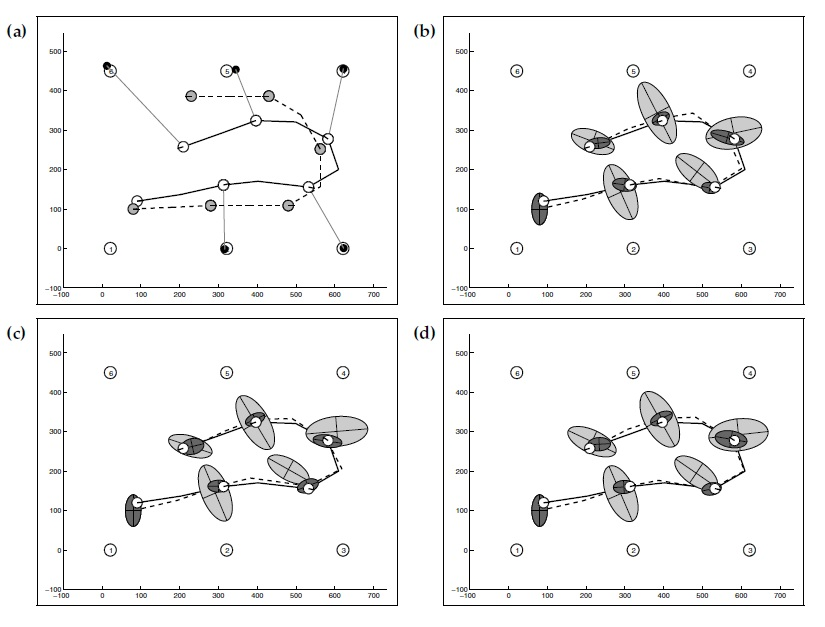
\includegraphics[width=1\linewidth]{715orig}}
	\caption{ (  Рис. 7.15 Сравнение оценок UKF и EKF: (a) Траектория робота согласно сигналам управления движением (пунктирные линии) и результирующая истинная траектория (сплошные линии). Обнаружения ориентиров показаны тонкими линиями. (b) Справочные оценки, сгенерированные многочастичным фильтром. Оценки EKF (c) и UKF (d).)}
	\label{fig:715orig}
\end{figure}

Влияние улучшенного алгоритма линеаризации, использованного в UKF, явно видно в примере, показанном на Рис. 7.16. Здесь робот выполняет две команды перемещения по кругу, изображённому тонкой линией. На графиках показаны эллипсы неопределённости после двух передвижений (робот не выполняет наблюдений). Ковариации, извлеченные из точных, основанных на выборке, обновлений движения, показаны для сравнения. Эталонные примеры были сгенерированы, используя алгоритм \textbf{sample\_motion\_model\_velocity} из Таблицы 5.3. Хотя линеаризация EKF приводит к существенным ошибкам как в местоположении среднего, так и в «форме» ковариации, оценки UKF практически идентичны эталонным. В этом примере также видна небольшая разница между прогнозами EKF и UKF. Математическое ожидание, прогнозируемое EKF, всегда точно обозначает местоположение, прогнозируемое на основании данных управления (строка 6 в таблице 7.2). С другой стороны, математическое ожидание UKF извлекается из сигма-точек и может отличаться от математического ожидания управления (строка 7 в Таблице 7.4).

\begin{figure}[H]
	\center{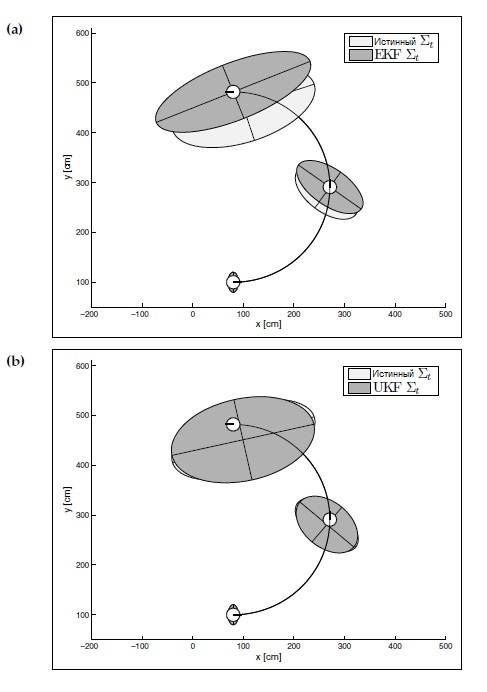
\includegraphics[width=0.85\linewidth]{716orig}}
	\caption{ ( Рис. 7.16 Ошибка аппроксимации, вызванная линеаризацией при движении робота по кругу. Оценки основываются на прогнозе EKF (a) и прогнозе UKF (b). Эталонные ковариации извлечены из точного прогноза на основе выборки. )}
	\label{fig:716orig}
\end{figure}

\textbf{7.8 Практические соображения}\\

Алгоритм локализации EKF и его близкий вариант, локализация MHT, являются популярными методами отслеживания позиции. Существует большое количество вариантов этих алгоритмов, улучшающих эффективность и надёжность. \\

•\textbf{ Эффективный поиск.} Во-первых,  перебор в цикле всех ориентиров $k$ на карте, как это выполняется в алгоритме локализации EKF с неизвестным соответствием часто оказывается непрактичным. Существуют довольно простые способы идентификации подходящих ориентиров (например, можно просто проектировать измерение в пространство $x-y$), позволяющие отбросить все ориентиры, кроме конечного постоянного числа специально отобранных.
Такие алгоритмы могут быть на порядки быстрее своих «наивных» реализаций.\\

• Взаимное исключение. Ключевое ограничение нашей реализации (которое наследуется и в MHT) возникает из-за предполагаемой независимости шумов признаков в EKF. Читатель может вспомнить условие (7.16), позволяющее последовательно обрабатывать отдельные признаки, что предотвращает возникновение операции поиска с экспоненциальной сложностью в пространстве всех векторов соответствия.
К сожалению, такой подход позволяет назначить несколько наблюдаемых признаков, скажем $z_t^i$ и $z_t^j$ с $i\neq j$, одному и тому же ориентиру $\hat{c}_t^i=\hat{c}_t^j$ на карте. Для многих датчиков такое назначение признаков по умолчанию неверно. Например, если вектор признаков извлекается из единичного изображения с камеры, точно известно, что два различных региона пространства изображения должны соответствовать разным местоположениям физического мира.
Другими словами, обычно известно, что $i\neq j\longrightarrow\hat{c}_t^i\neq\hat{c}_t^j$.\\
ПРИНЦИП ВЗАИМНОГО ИСКЛЮЧЕНИЯ ПРИ АССОЦИАЦИИ ДАННЫХ\\
Это (жёсткое!) ограничение называется принципом взаимного исключения при ассоциации данных. Оно позволяет уменьшает пространство всех возможных векторов соответствия и учитывается в хороших реализациях алгоритма. Например, можно сначала раздельно искать каждое соответствие, как в нашей версии локализации EKF, а затем выполнить «ремонтный» проход, в котором будут выявлены и устранены нарушения принципа взаимного исключения с помощью изменения значений соответствия.\\

• Вычёркивание выбросов. Далее, в предложенной реализации не обрабатываются выбросы. Читатель может вспомнить, что в подразделе 6.6 для соответствия было разрешено лишь $c = N + 1$ ориентиров, где $N$ - общее число ориентиров на карте. Такой тест на выбросы довольно легко добавляется к алгоритмам локализации EKF. В частности, если установить $\pi_{N+1}$ как априорную вероятность выброса, операция argmax в строке 16 локализации EKF (Таблица 7.3) может по умолчанию иметь значение $N +1$, если наиболее вероятным объяснением вектора измерения является выброс. Вообще-то, выброс не содержит никакой информации о положении робота, поэтому все члены выражения в строках 18 и 19 в Таблице 7.3, имеющие отношение к положению, просто вычёркиваются.\\

Для задач отслеживания позиции применимы только локализации EKF и UKF.
В общем, методы линеаризованных гауссовых функций хорошо работают только при малой неопределённости позиции. Это утверждение основано на нескольких взаимодополняющих факторах:\\

• Одномодальный гауссиан обычно является хорошим представлением неопределённости при отслеживании, если оно не входит в более глобальную задачу локализации.\\

• Даже при отслеживании позиции одномодальные гауссианы плохо подходят для отображения жёстких пространственных ограничений вида «робот может быть близко к стене, но не может находиться внутри неё». Значимость этих ограничений возрастает с ростом неопределённости местоположения робота.\\

• Узкий гауссиан уменьшает опасность ошибочного назначения соответствия. Это особенно важно для EKF, поскольку единственное неверное соответствие может дезориентировать трекер, вызвав целый поток ошибок локализации и соответствия. \\

• Линеаризация обычно хорошо работает только вблизи точки линеаризации. Как правило, если стандартное отклонение ориентации $\theta$ превышает $\pm20$ градусов, эффекты линеаризации, скорее всего, приведут к отказу как EKF, так и UKF алгоритмов.\\

В алгоритме MHT большинство этих проблем решены, правда, ценою увеличенной вычислительной сложности.\\

• С его помощью можно решить проблему глобальной локализации, инициализировав начальную гипотезу несколькими гауссовыми гипотезами. Гипотезы могут быть инициализированы по первым измерениям.\\

• Проблема похищенного робота может быть решена добавлением в смесь новых гипотез.\\

• Жёсткие пространственные ограничения так же трудно моделировать, но их можно лучше аппроксимировать несколькими гауссианами. \\

• Алгоритм MHT более надёжен при ошибках соответствия, хотя может отказать, если верное соответствие среди сохранённых в смеси гауссианов отсутствует.\\

• Обсуждаемый алгоритм MHT использует ту же самую линеаризацию, что и EKF, страдая от аналогичных негативных эффектов аппроксимации. Алгоритм MHT также возможно реализовать, используя UKF для каждой из гипотез.\\

Разработка подходящих признаков для алгоритмов гауссовой локализации является, в некотором роде, искусством. Это происходит потому, что необходимо достичь нескольких взаимоисключающих целей. 
С одной стороны, хочется иметь достаточно много признаков в среде, чтобы сохранить малую степень неопределённости положения робота, которая абсолютно необходима в силу указанных выше причин. С другой стороны, желательно минимизировать шансы перепутать ориентиры друг с другом, или  ошибочного обнаружения признака. Во многих средах не так много точечных ориентиров, которые можно надёжно распознать, поэтому, зачастую, в реализациях предполагаются достаточно свободно распределённые ориентиры. Здесь у алгоритма MHT есть явное преимущество в силу большей надёжности при ошибках ассоциации данных. Как правило, большое количество ориентиров работает лучше даже для EKF и UKF. При плотном расположении ориентиров критически важно использовать взаимное исключение при ассоциации данных. 

Наконец, заметим, что в процессе локализации в EKF и UKF обрабатываесят только часть информации измерения. При переходе от измерений к признакам количество обрабатываемой информации и так сильно уменьшается.\\
ОТРИЦАТЕЛЬНАЯ ИНФОРМАЦИЯ\\ Более того, ни EKF, на UKF методы локализация неспособны обрабатывать отрицательную информацию, указывающую на отсутствие признака. Очевидно, что отсутствие признака там, где он должен быть, является релевантной информацией. Например, если из какого-то места в Париже не видна Эйфелева башня, очень маловероятно, что это место расположено близко к ней. Проблема отрицательной информации состоит в том, что она порождает негауссовы гипотезы, которые невозможно представить в виде математического ожидания и дисперсии. Именно поэтому в реализациях EKF и UKF отрицательная информация просто игнорируется, а учитывается только информация от обнаруженных признаков. Стандартный алгоритм MHT также не учитывает отрицательной информации. Однако, её можно включить в вес смеси, разложив компоненты, для которых не удалось обнаружить ориентир.

Учитывая все ограничения, не означает ли это, что методы локализации на основе гауссианов ненадёжны? Ответ - нет. EKF,  UKF, и, особенно, MHT удивительно устойчивы к нарушениям допущений линейных систем. Фактически, успешная локализация зависит только от успешной ассоциации данных. Позже в книге мы столкнёмся с более сложными методами обработки соответствия, нежели только что обсуждаемые. 
Многие из этих методов применялись (и будут применяться) к нормальным распределениям, и результирующие алгоритмы относятся к лучших из известных ныне.\\

\textbf{7.9 Выводы} \\

В этой главе была представлена проблема локализации мобильного робота и выведен первый практический алгоритм ее решения.\\

• Проблема локализации состоит в оценке положения робота относительно известной карты окружающей среды.\\

• Отслеживание позиции относится к проблемам обработки локальной неопределённости положения робота, с известным начальным положением. Глобальная локализация - более общая проблема локализации робота «с нуля». Проблема похищенного робота – это проблема локализации в которой робот, имеющий данные о своём местоположении, мгновенно переносится в другое место. Эта проблема является самой трудной. \\

• Трудность проблемы локализации также является функцией изменчивости окружающей среды со временем. Все обсуждаемые алгоритмы подразумевают статическую окружающую среду.\\

• Пассивные методы локализации основаны на использовании фильтров. В них обрабатываются данных, полученные роботом, но отсутствует вмешательство в управление роботом. Методы активной локализации управляют роботом при локализации с целью минимизировать неопределённость. До настоящего момента изучались только пассивные алгоритмы. Активные алгоритмы будут обсуждаться в Главе 17.\\

• Марковская локализация является просто другим названием фильтра Байеса, применённого для проблемы локализации мобильного робота. \\

• Локализация на основе EKF использует обобщенный фильтр Калмана и используется, в основном,  для карт на основе признаков.\\

• Самый часто используемый метод  решения проблемы соответствия, это метод максимального правдоподобия. Этот метод подразумевает, что в каждый момент времени истинно самое  соответствие с наибольшей вероятностью.\\

• Алгоритм отслеживания нескольких гипотез (MHT) для представления апостериорного распределения использует несколько соответствий в виде смеси гауссовых функций. Компоненты смеси создаются динамически и уничтожаются, если их общее правдоподобие падает ниже порогового значения, определённого пользователем. \\

• MHT более устойчив к проблемам ассоциации данных, чем EKF, но за счёт увеличения вычислительной сложности. MHT также возможно реализовать, используя UKF для отдельных гипотез.\\

• Локализация UKF использует unscented преобразование для линеаризации моделей движения и измерения в контексте проблемы локализации.\\

• Все гауссовы фильтры хорошо подходят для задач отслеживания локальной позиции с ограниченной неопределённостью и в средах с явно различимыми признаками. EKF и UKF менее применимы для глобальной локализации или для сред с множеством схожих объектов. \\

• Отбор признаков для гауссовых фильтров требует навыка. Признаки должны быть достаточно уникальными, чтобы уменьшить шансы перепутать их, но их должно быть достаточно много, чтобы робот  обнаруживал признаки достаточно часто. \\

• Производительность гауссовых алгоритмов локализации может быть улучшена различными способами, такими как принудительное взаимное исключение при ассоциации данных. \\

В следующей главе будут обсуждаться альтернативные методы локализации, направленные на обход ограничений EKF, используя различные представления гипотезы робота. \\

\textbf{7.10 Библиографические примечания}\\

Локализация была названа «самой фундаментальной проблемой для создания мобильного робота с возможностями автономности» (Cox, 1991). Использование EKF для оценки состояния роботов, действующих вне помещений впервые было выполнено Дикманнсом и Грэфи (Dickmanns and Graefe, 1988), которые применили EKF для оценки кривизны дороги по изображениям с камеры. Большая часть ранних работ по локализации мобильных роботах в помещениях была описана Боренштейном (Borenstein et al.,1996) (см. также (Feng et al., 1994)). Кокс и Вилфонг (Cox and Wilfong, 1990) представили ранний текст о наиболее современных на тот момент разработках в мобильной робототехнике, включив в него локализацию. Многие ранние методы требовали модификации окружающей среды, например, с помощью искусственных меток. Например, Леонард и Дюран-Уайт (Leonard and Durrant-Whyte, 1991) использовали EKF при сравнении геометрических маркеров, извлекая данные о них из показаний сонара, и используя бакены, расположенные с учётом геометрической карты окружающей среды. Практика использования искусственных маркеров сохранилась до сегодняшнего дня (Salichs et al, 1999), поскольку  модификация окружающей среды часто оправдана и выгодна. Другие исследователи применяли лазеры для сканирования не модифицированных сред (Hinkel and Knieriemen, 1988).

Уходя от точечных признаков, некоторые исследователи разработали новые геометрические методы локализации. Например, Кокс (Cox, 1991) разработал алгоритм  сравнения расстояний, измеренных инфракрасными датчиками, и описания окружающей среды в виде совокупности линейных сегментов. Метод, разработанный Вейсом (Weiss et al., 1994) использовал корреляцию измерений расстояния для локализации. Идея наложения карт, особенно, сравнения локальной карты сетки занятости с глобальной картой среды, принадлежит Моравицу ( Moravec, 1988). Метод локализации градиентным спуском на базе этой идеи был описан Труном (Thrun, 1993), и использован в первом соревновании AAAI в 1992 году (Simmons et al. 1992). Шили и Краули (Schiele and Crowley, 1994) выполнили сравнение различных стратегий отслеживания позиции робота на основе карт сеток занятости с помощью ультразвуковых датчиков. Они показали, что наложение локальных карт сеток занятости на глобальную карту с сеткой показывает схожую производительность с наложением на основе признаков, извлечённых из обеих карт. Шаффер (Shaffer et al., 1992) сравнил устойчивость наложения карт и методов на основе признаков и показал, что комбинация обоих показывает лучшие эмпирические результаты. Ямаучи и Лэнгли (Yamauchi and Langley, 1997) доказали устойчивость наложения карт к изменениям среды. Идея использования наложения проходов сканирования для локализации в робототехнике восходит к работам Лю и Милиоса (Lu and Milios, 1994, 1998), Гутмана и Шлегеля (Gutmann and Schlegel, 1996), хотя базовый принцип был популярен и в других областях (Besl and McKay 1992). Похожий метод был предложен Аррасом и Вестли (Arras and Vestli, 1998), которые показали, что, используя наложение проходов сканирования, возможно локализовать робота с исключительной точностью. Ортин (Ortin et al., 2004) обнаружил, что использование соечтания камеры с лазерным дальномером увеличивает устойчивость наложения измерений расстояния.

Другая ветвь исследований была посвящена геометрическим методам локализации (Betke and Gurvits 1994). Термин «проблема похищенного робота» принадлежит Энгельсону и МакДермотту (Engelson and McDermott, 1992). Название «марковская локализация» было введено Симмонсом и Кёнигом (Simmons and Koenig, 1995), которые предложили алгоритм локализации с сеткой для отображения апостериорных вероятностей. Однако, корни этой работы восходят к Норбахшу (Nourbakhsh et al., 1995), который разработал идею «коэффициентов уверенности» для локализации мобильного робота. Хотя правила обновления для коэффициентов уверенности не следовали строго теоремам вероятности, в них была отражена важная идея оценки нескольких гипотез. В основополагающей работе Кокса и Леонарда (Cox and Leonard, 1994) эта идея также была исследована в виде динамически поддерживаемых деревьев гипотез локализации робота. Использование нечёткой логики для локализации робота было предложена Саффотти (Saffiotti, 1997).  Также можно обратиться к работам Дрянкова и Саффиотти (Driankov and Saffiotti, 2001).\\

\textbf{7.11 Упражнения}\\

1. Допустим, робот оснащён датчиком для измерения расстояния и направления на ориентир. Для простоты допустим, что при измерении робот распознаёт  и обозначение ориентира (датчик определения ориентира идеальный и не подвержен шумам). Требуется выполнить глобальную локализацию, используя EKF. Обратить внимание, что при обнаружении одиночного ориентира апостериорная вероятность обычно плохо аппроксимируется с помощью гауссовой функции. Однако, при обнаружении двух и более ориентиров одновременно, апостериорное распределение хорошо приближается с помощью гауссиана.\\

(a) Объяснить, почему это происходит.\\

(b) Даны $k$ одновременных измерений расстояния и направления для $k$ опознаваемых ориентиров. Разработать процедуру вычисления гауссовой оценки положения робота с равномерным начальным априорным распределением. Следует начать с модели измерения расстояния/направления, представленной в подразделе 6.6.\\

2. В этом упражнении потребуется создать жёсткие окружающие среды для глобальной локализации. Допустим, необходимо составить плоскую окружающую среду из $n$ непересекающихся прямых отрезков. Свободное пространство среды замкнуто, но внутри карты может быть замкнутый островок занятой территории. Для этого упражнения допустим, что робот оснащён круговым массивом из 360 датчиков расстояния, датчики идеальны и их показания всегда точны.\\

(a) Каково максимальное количество отдельных модов в функции оценки может встретиться при глобальной локализации? Для $n = 3, . . . , 8$ нарисовать среды, вызывающие наибольшие трудности, вместе с применимой гипотезой, максимизирующей количество модов.\\

(b) Изменится ли алгоритм анализа, если разрешить датчикам расстояния ошибаться? В частности, дать пример для $n = 4$, с большим количеством  правдоподобных модов, чем в примере выше. Показать такую среду, обозначив (ложные) показания расстояния и апостериорное распределение.\\ 
3. Требуется вывести алгоритм локализации EKF для простейшего подводного робота. Робот находится в трехмерном пространстве и оснащён идеальным компасом (то есть ориентация по направлению всегда известна). Для простоты допустим, что робот движется независимо по всем трём перпендикулярным осям $(x, y, z)$, управляя скоростями $\dot{x},\dot{y},\dot{z}$. Шумы движения выражены нормальными распределениями и независимы по всем трём направлениям.

Робот окружен некоторым количеством бакенов, которые излучают акустические сигналы. Время момента включения каждого сигнала известно, но робот способен по сигналу определить, каким именно бакеном он был излучён (поэтому проблемы соответствия данных нет). Робот также знает местонахождение всех бакенов и оснащён точным хронометром для замера времени прохождения каждого сигнала. Однако, робот неспособен определить направление, с которого был получен сигнал. \\

(a) Необходимо вывести алгоритм локализации о робота на основе EKF.
Это включает математический вывод моделей движения и измерения, а также аппроксимацию разложением в ряд Тейлора. Также необходимо определить финальный алгоритм на основе EKF с известным соответствием.
\\

(b) Реализовать алгоритм на основе EKF и имитацию среды.
Проверить точность и режимы отказов алгоритма локализации EKF в контексте трёх проблем локализации: глобальной локализации, отслеживания позиции и проблемы похищенного робота.\\

4. Представить упрощённую глобальную локализацию в любой из шести следующих сред с наложенной сеткой:

\begin{figure}[H]
	\center{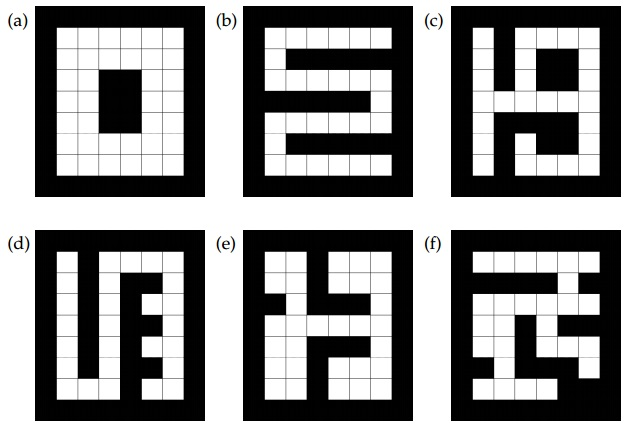
\includegraphics[width=0.9\linewidth]{717orig}}
	\label{fig:717orig}
\end{figure}

В каждой среде робот размещается в случайном месте, ориентированный по направлению на север. Требуется вывести локализацию без обратной связи, которая будет содержать последовательность следующих команд:\\

\textit{Действие L: Повернуть налево на 90 градусов.}

\textit{Действие R: Повернуть направо на 90 градусов.}

\textit{Действие M: Двигаться вперёд до столкновения с препятствием.}\\

В конце стратегии робот должен оказаться в определимой позиции.
Для каждой такой среды представить кратчайшую последовательность (считать только действия “M”). Указать, в каком месте окажется робот после окончания последовательности действий. Если такой последовательности не существует, объяснить, почему.\\

5. Теперь допустим, что робот способен считать количество шагов после выполнении команды “M” из предыдущего упражнения. Какова будет кратчайшая последовательность для определения местоположения? Объяснить ответ.\\

Примечание: В этом вопросе может оказаться, что конечное местоположение робота является функцией начального положения. Требуется только выполнить локализацию робота.\\




 
\end{document}